\documentclass[11pt]{article}
\usepackage[utf8]{inputenc}
\usepackage[T1]{fontenc}
\usepackage[spanish,es-tabla]{babel}
\usepackage{graphicx}
\graphicspath{ {images/} }
\usepackage{float}
\usepackage[margin=2cm]{geometry}
\usepackage{fancyhdr}
\usepackage{caption}
\usepackage{setspace}
\usepackage{amsmath}
\usepackage{amssymb}
\usepackage{titlesec}
\usepackage[table,xcdraw]{xcolor}
\usepackage{listings}
\usepackage{url}
\usepackage{tikz}
\usetikzlibrary{shapes.geometric, arrows, calc, decorations.pathreplacing, positioning, babel}

% Color institucional IBERO
\definecolor{iberoblue}{HTML}{003087}

\lstset{
    breaklines=true,
    breakatwhitespace=true,
    keepspaces=true,
    breakindent=0pt,
    postbreak=\mbox{\textcolor{red}{$\hookrightarrow$}\space},
}

\definecolor{mlblue}{rgb}{0.0, 0.0, 0.55}
\definecolor{mlpurple}{rgb}{0.6, 0.1, 0.6}
\definecolor{mlcomment}{rgb}{0.30, 0.50, 0.30}

% Lenguaje JavaScript para listings (no viene predefinido)
\lstdefinelanguage{JavaScript}{
  keywords={const, let, var, function, return, if, else, for, of, in, new, export, import, from, break, continue},
  sensitive=true,
  comment=[l]{//},
  morecomment=[s]{/*}{*/},
  morestring=[b]',
  morestring=[b]",
  morestring=[b]`
}

\lstdefinestyle{js}{
  language=JavaScript,
  basicstyle=\ttfamily\small,
  keywordstyle=\color{mlblue}\bfseries,
  commentstyle=\color{mlcomment}\itshape,
  stringstyle=\color{mlpurple},
  numbers=left,
  numberstyle=\tiny\color{gray},
  stepnumber=1,
  numbersep=5pt,
  backgroundcolor=\color{gray!10},
  showspaces=false,
  showstringspaces=false,
  showtabs=false,
  frame=single,
  rulecolor=\color{black},
  tabsize=2,
  captionpos=b,
  breaklines=true,
  breakatwhitespace=false
}

% Mismo estilo visual para Python
\lstdefinestyle{py}{
  style=js,
  language=Python,
  morekeywords={self, True, False, None},
}

\titlespacing*{\section}{0pt}{12pt}{6pt}
\titlespacing*{\subsection}{0pt}{12pt}{6pt}
\setlength{\parskip}{0.5em}

\pagestyle{fancy}
\fancyhf{}
\renewcommand{\headrulewidth}{0pt}
\fancyfoot[C]{\thepage}

\title{\textbf{Aprendizaje reforzado: SARSA, Q-learning y Deep Q-learning\\El Paso del Contrabandista y el alunizaje con DQN}}
\author{Carlos Ortega}
\date{\today}

\begin{document}

% ============================================================
%  LOGO DE INGENIERIA
%  Coloca el archivo en:  images/IBERO-IE.png  (o .pdf / .jpg)
% ============================================================
\begin{figure}[t]
\centering

\includegraphics[width=0.4\textwidth]{images/IBERO-IE}
\end{figure}

\vspace{1cm}

\maketitle
\thispagestyle{fancy}

\begin{center}
\large{\textbf{Universidad Iberoamericana}}\\
\large{Ingeniería en Mecatrónica y Sistemas Ciberfísicos}\\
\large{Control Inteligente}\\
\large{Otoño 2026}\\
\end{center}

\section*{Introducción}

El objetivo de esta práctica es analizar y comparar el \textbf{comportamiento de
riesgo} de una política \emph{on-policy} (SARSA) y una \emph{off-policy}
(Q-learning) en una tarea de navegación táctica con incertidumbre, y después
escalar a un espacio de estados continuo con \textbf{Deep Q-Learning} (DQN).

El primer ejercicio simula un robot móvil con ocho grados de libertad de
movimiento en una malla de $20 \times 20$ con obstáculos y piso resbaloso. Se
diseñó el mapa \emph{El Paso del Contrabandista}: una barrera vertical separa el
inicio A de la meta B y solo tiene una \textbf{brecha de una celda}, que se cruza
en diagonal (camino corto y peligroso), mientras que un espacio abierto permite
rodear la barrera (camino largo y seguro). La pregunta central es cuál de las dos
rutas aprende cada algoritmo y por qué. El tema visual del sitio es americanista:
el robot \emph{busca el gol}, cada episodio es un \emph{partido} y cada choque es
una \emph{tarjeta roja}.

El segundo ejercicio entrena un agente DQN en el entorno \texttt{LunarLander} de
Gymnasium, cuyo estado $s \in \mathbb{R}^8$ es continuo, para aterrizar un módulo
entre dos banderas. Se estudian sus fases de aprendizaje, el efecto de la
penalización por combustible y la escalabilidad de una tabla Q frente a una red
neuronal.

El procedimiento seguido fue: modelar ambos problemas como MDP, implementar los
agentes en Python (NumPy y PyTorch), entrenarlos localmente en CPU con varias
semillas, exportar los resultados y publicarlos en un sitio web interactivo con
despliegue automático en GitHub Pages. El sitio incluye dos juegos 3D: uno donde
SARSA y Q-learning juegan el mismo partido con sus tablas Q reales, y otro donde
la red DQN entrenada en Python pilota el módulo lunar directamente en el
navegador.

\noindent Sitio: \url{https://sebastiux.github.io/practiva7inteligente/}\\
Repositorio: \url{https://github.com/sebastiux/practiva7inteligente}

\section{Especificaciones de diseño}

\begin{table}[H]
\centering
\renewcommand{\arraystretch}{1.2}
\begin{tabular}{|l|c|c|}
\hline
\rowcolor{iberoblue}\textcolor{white}{\textbf{Parámetro (Ejercicio 1)}} & \textcolor{white}{\textbf{En la práctica}} & \textcolor{white}{\textbf{Valor usado}} \\ \hline
Estados $\mathcal{S}$                  & malla $N \times N$ (sugerido $20 \times 20$) & $20 \times 20 = 400$ celdas \\ \hline
Acciones $\mathcal{A}$                 & $\{N, S, E, O, NE, NO, SE, SO\}$ & 8 acciones \\ \hline
Resbalamiento $p_{\text{slip}}$        & $0.1$                           & $0.1$ \\ \hline
Recompensa por llegar a la meta        & $+100$                          & $+100$ (termina) \\ \hline
Colisión con obstáculo o pared         & $-100$ (termina)                & $-100$ (termina) \\ \hline
Paso cardinal / diagonal               & $-1.0$ / $-1.41$                & $-1.0$ / $-1.41$ \\ \hline
Tasa de aprendizaje $\alpha$           & $0.1$                           & $0.1$ \\ \hline
Factor de descuento $\gamma$           & $0.9$                           & $0.9$ \\ \hline
Exploración $\varepsilon$              & $0.1$ (constante)               & $0.1$ (constante) \\ \hline
Episodios                              & $5{,}000$--$10{,}000$           & $10{,}000$ \\ \hline
Semillas                               & no especificado                 & $5$ (de la 0 a la 4) \\ \hline
Límite de pasos por episodio           & no especificado                 & $400$ (truncamiento) \\ \hline
\end{tabular}
\caption{Parámetros del Ejercicio 1 (SARSA y Q-learning).}
\label{tbl:especificaciones1}
\end{table}

\begin{table}[H]
\centering
\renewcommand{\arraystretch}{1.2}
\begin{tabular}{|l|c|c|}
\hline
\rowcolor{iberoblue}\textcolor{white}{\textbf{Parámetro (Ejercicio 2)}} & \textcolor{white}{\textbf{En la práctica}} & \textcolor{white}{\textbf{Valor usado}} \\ \hline
Entorno                                & \texttt{LunarLander-v2}          & \texttt{LunarLander-v3} \\ \hline
Red neuronal                           & 2 ocultas de 64 o 128           & $8 \to 128 \to 128 \to 4$ \\ \hline
Activación de las capas ocultas        & ReLU                            & ReLU \\ \hline
Tasa de aprendizaje $\alpha$ (Adam)    & $0.0005$                        & $0.0005$ \\ \hline
Factor de descuento $\gamma$           & $0.99$                          & $0.99$ \\ \hline
Exploración $\varepsilon$              & $1.0 \to 0.01$                  & $\times 0.995$ por episodio, mín. $0.01$ \\ \hline
Episodios                              & $600$--$1{,}000$                & máx. $1{,}000$ (paro: media $\ge 200$) \\ \hline
Experience Replay                      & sí                              & buffer de $100{,}000$, lote de $64$ \\ \hline
Red objetivo                           & no especificada                 & actualización suave, $\tau = 10^{-3}$ \\ \hline
Frecuencia de aprendizaje              & no especificada                 & cada $4$ pasos \\ \hline
Evaluación                             & política greedy ($\varepsilon = 0$) & $20$ episodios \\ \hline
\end{tabular}
\caption{Parámetros del Ejercicio 2 (DQN). \texttt{LunarLander-v2} ya no existe
en Gymnasium 1.4; la versión 3 conserva el mismo estado, las mismas acciones y la
misma recompensa, con correcciones de errores.}
\label{tbl:especificaciones2}
\end{table}

\section{Marco teórico}

\subsection{Procesos de decisión de Markov}

Un MDP es la tupla $(\mathcal{S}, \mathcal{A}, P, R, \gamma)$: en cada paso $t$
el agente observa $S_t$, elige $A_t$, recibe $R_{t+1}$ y pasa a $S_{t+1}$ con
probabilidad $P(s' \mid s, a)$. Se cumple la \emph{propiedad de Markov}: el
futuro depende solo del estado actual. El objetivo es maximizar el
\textbf{retorno descontado}
\begin{equation}
G_t = \sum_{k=0}^{\infty} \gamma^k R_{t+k+1}, \qquad 0 \le \gamma < 1,
\label{eq:retorno}
\end{equation}
y la función de acción-valor $Q_\pi(s,a) = \mathbb{E}_\pi[G_t \mid S_t = s, A_t = a]$
mide qué tan buena es la acción $a$ en el estado $s$ si después se sigue $\pi$.

\subsection{Aprendizaje por diferencias temporales}

Los métodos de diferencias temporales (TD) aprenden $Q$ sin conocer $P$,
corrigiendo la estimación paso a paso hacia un \emph{blanco} que combina la
recompensa inmediata con el valor estimado del estado siguiente. La exploración
se resuelve con una política $\varepsilon$-greedy: con probabilidad
$1-\varepsilon$ se elige $\arg\max_a Q(s,a)$ y con probabilidad $\varepsilon$
una acción al azar.

\begin{itemize}
    \item \textbf{Q-learning (off-policy)} aprende el valor de la política óptima
    independientemente de las acciones exploratorias que tome:
    \begin{equation}
    Q(s,a) \leftarrow Q(s,a) + \alpha\Big[r + \gamma \max_{a'} Q(s',a') - Q(s,a)\Big].
    \label{eq:qlearning}
    \end{equation}
    \item \textbf{SARSA (on-policy)} aprende el valor de la política que
    realmente ejecuta, exploración incluida, porque usa la acción $a'$ que la
    política $\varepsilon$-greedy sí elegirá en $s'$:
    \begin{equation}
    Q(s,a) \leftarrow Q(s,a) + \alpha\Big[r + \gamma\, Q(s',a') - Q(s,a)\Big].
    \label{eq:sarsa}
    \end{equation}
\end{itemize}
La única diferencia entre (\ref{eq:qlearning}) y (\ref{eq:sarsa}) es el término
del estado siguiente: $\max_{a'}Q(s',a')$ contra $Q(s',a')$. Esa diferencia
determina la actitud de cada algoritmo ante el riesgo: Q-learning valora cada
estado suponiendo que en el futuro siempre jugará la mejor acción, mientras que
SARSA incorpora la probabilidad real de equivocarse al explorar.

\subsection{Deep Q-learning}

Cuando el estado es continuo, la tabla Q es inviable. DQN la reemplaza por una
red neuronal con pesos $w$,
\begin{equation}
Q(s,a) \approx Q(s,a; w),
\label{eq:aprox}
\end{equation}
entrenada por retropropagación para minimizar el error cuadrático contra el
blanco de Bellman:
\begin{equation}
\mathcal{L}(w) = \mathbb{E}\Big[\big(r + \gamma \max_{a'} Q(s',a'; w^-) - Q(s,a;w)\big)^2\Big].
\label{eq:loss}
\end{equation}
Se usan dos mejoras estándar sobre la formulación básica:
\begin{itemize}
    \item \textbf{Experience Replay:} las transiciones $(s, a, r, s', \text{terminal})$
    se guardan en un buffer circular y se entrena con mini-lotes aleatorios, lo
    que rompe la correlación temporal entre muestras consecutivas y reutiliza la
    experiencia.
    \item \textbf{Red objetivo:} la ecuación (4) de la práctica usa los mismos
    pesos $w$ en el blanco y en la predicción, por lo que el blanco se mueve con
    cada paso de gradiente. Aquí el blanco se calcula con una copia lenta $w^-$
    actualizada suavemente, $w^- \leftarrow \tau w + (1-\tau) w^-$ (Mnih et al.,
    2015). No es parte del enunciado, pero estabiliza mucho el entrenamiento.
\end{itemize}

\section{Modelado del problema}

\subsection{MDP del Grid World 8-DOF}

\begin{itemize}
    \item \textbf{Estados:} las $400$ celdas $s = (\text{fila}, \text{columna})$.
    La barrera ocupa la columna $10$ de la fila $0$ a la $11$, con la brecha en
    $(6, 10)$. El inicio es $A = (4, 6)$ y la meta $B = (7, 15)$; las filas $12$ a
    $19$ forman el espacio abierto para rodear (Figura~\ref{fig:mapa}).
    \item \textbf{Acciones:} 4 cardinales y 4 diagonales.
    \item \textbf{Transición con resbalamiento:} con probabilidad $0.9$ el robot va
    a donde quiso; con probabilidad $0.1$ patina y cae, con la misma probabilidad,
    en la dirección girada $-45^\circ$, en la girada $+45^\circ$ (celdas
    adyacentes a la deseada) o se queda en su lugar:
    \begin{equation}
    P(s' \mid s, a) =
    \begin{cases}
    0.9 & s' = s + \Delta(a)\\
    0.1/3 & s' \in \{\, s + \Delta(a_{-45^\circ}),\; s + \Delta(a_{+45^\circ}),\; s \,\}
    \end{cases}
    \label{eq:slip}
    \end{equation}
    \item \textbf{Recompensa:} $+100$ al llegar a B, $-100$ al chocar (el robot no
    avanza y el episodio termina), $-1$ por paso cardinal y $-1.41$ por paso
    diagonal. El costo se cobra según la acción \emph{comandada}, aunque el robot
    patine.
    \item \textbf{Regla de colisión diagonal (decisión de diseño):} un movimiento
    choca solo si la celda \emph{destino} es un obstáculo o queda fuera de la
    malla. Una diagonal puede pasar rozando las esquinas de dos obstáculos. Por eso
    la brecha se cruza en diagonal, $(5,9) \xrightarrow{SE} (6,10) \xrightarrow{SE} (7,11)$,
    y por eso mismo es peligrosa: dentro de ella, una acción exploratoria hacia
    el norte o el sur termina en la barrera.
\end{itemize}

\begin{figure}[H]
\centering
\begin{tikzpicture}[>=stealth, cell/.style={draw=gray!60, minimum size=1.1cm, inner sep=0pt}]
\foreach \x in {0,1,2} \foreach \y in {0,1,2} \node[cell] at (\x*1.1,\y*1.1) {};
\node[cell, fill=iberoblue!15] (s) at (1.1,1.1) {};
\node[cell, fill=yellow!40] (ne) at (2.2,2.2) {};
\node[cell, fill=yellow!15] (n)  at (1.1,2.2) {};
\node[cell, fill=yellow!15] (e)  at (2.2,1.1) {};
\node[font=\bfseries] at (0.85,0.85) {$s$};
\draw[->, very thick, iberoblue] (s.center) -- (ne.center);
\draw[->, thick, red!70!black] (s.center) -- (n.center);
\draw[->, thick, red!70!black] (s.center) -- (e.center);
\draw[->, thick, red!70!black] (1.3,0.8) arc (-60:250:0.2);
\node[font=\scriptsize, iberoblue, anchor=west] at (2.8,2.2) {$0.9$: NE (pedida)};
\node[font=\scriptsize, red!70!black, anchor=south] at (1.1,2.8) {$0.1/3$: N};
\node[font=\scriptsize, red!70!black, anchor=west] at (2.8,1.1) {$0.1/3$: E};
\node[font=\scriptsize, red!70!black, anchor=east] at (-0.6,1.1) {$0.1/3$: se queda en $s$};
\end{tikzpicture}
\caption{Modelo de resbalamiento para la acción NE: $0.9$ a la celda pedida y
$0.1/3$ a cada celda adyacente a la deseada (N, E) o permanecer en $s$.}
\label{fig:slip}
\end{figure}

\begin{figure}[H]
\centering
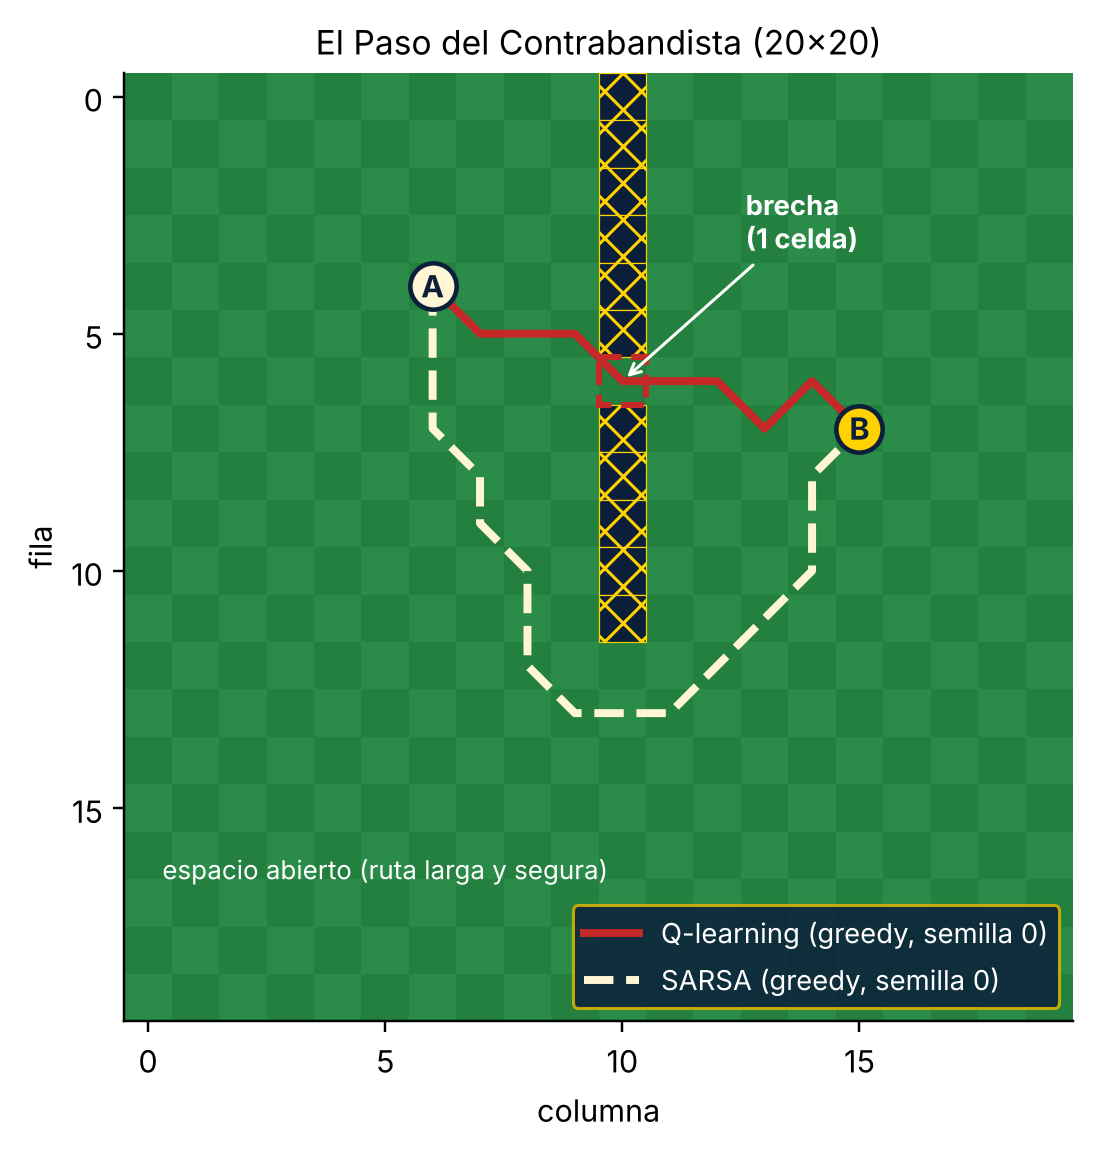
\includegraphics[width=0.58\textwidth]{images/mapa.png}
\caption{Mapa \emph{El Paso del Contrabandista}. En rojo, la ruta greedy aprendida
por Q-learning (cruza la brecha); en crema punteado, la de SARSA (rodea la
barrera). Ambas siguen la política final de la semilla 0 sin resbalones.}
\label{fig:mapa}
\end{figure}

El mapa se ajustó para que el dilema fuera real. Con $\gamma =
0.9$, el camino corto tiene mucho más valor descontado, pero la brecha
multiplica el riesgo: dentro de ella, el resbalón y la exploración pueden mandar
al robot contra la barrera. Con programación dinámica se verificó que la política
óptima greedy (la que aprende Q-learning) cruza la brecha y que la política
óptima $\varepsilon$-suave con $\varepsilon = 0.1$ (la que aprende SARSA) la
rodea.

\subsection{Ejemplo numérico de una actualización}

Con la tabla Q final de Q-learning (semilla 0), el robot está en $s = (5,9)$,
justo antes de la brecha, ejecuta $a = SE$, no resbala, llega a $s' = (6,10)$ y
paga $r = -1.41$. El valor actual es $Q(s,a) = 51.54$.

\begin{align*}
\textbf{Q-learning:}\quad & \max_{a'} Q(s',a') = Q(s', E) = 59.74,\\
& \text{blanco} = -1.41 + 0.9(59.74) = 52.36,\\
& Q(s,a) \leftarrow 51.54 + 0.1(52.36 - 51.54) = \mathbf{51.62}.\\[6pt]
\textbf{SARSA:}\quad & a' = N \text{ (acción exploratoria)},\quad Q(s', N) = -84.59,\\
& \text{blanco} = -1.41 + 0.9(-84.59) = -77.54,\\
& Q(s,a) \leftarrow 51.54 + 0.1(-77.54 - 51.54) = \mathbf{38.63}.
\end{align*}

Con la misma experiencia, Q-learning casi no cambia su valoración de entrar a la
brecha, mientras que SARSA la castiga, porque con $\varepsilon = 0.1$ de vez en
cuando sí jugará esa acción mala. Repetida miles de veces, esta diferencia es la
que separa las dos rutas.

\subsection{MDP de LunarLander}

\begin{itemize}
    \item \textbf{Estado} $s \in \mathbb{R}^8$: posición $(x, y)$, velocidades
    $(v_x, v_y)$, ángulo y velocidad angular $(\theta, \dot\theta)$ y contacto
    binario de cada pata $(l_{\text{izq}}, l_{\text{der}})$.
    \item \textbf{Acciones:} $\{0$: nada, $1$: propulsor izquierdo, $2$: motor
    principal, $3$: propulsor derecho$\}$.
    \item \textbf{Recompensa densa:} premia acercarse a la plataforma despacio y
    nivelado, $+10$ por cada pata en tierra, $+100$ por aterrizar, $-100$ por
    estrellarse, y penaliza el combustible con $-0.3$ por cuadro de motor
    principal y $-0.03$ por cuadro de propulsor lateral.
\end{itemize}

\begin{figure}[H]
\centering
\begin{tikzpicture}[>=stealth, neuron/.style={circle, draw=iberoblue, thick, minimum size=0.42cm, inner sep=0pt},
  lbl/.style={font=\scriptsize, align=center}]
\foreach \i in {1,...,8} \node[neuron, fill=yellow!20] (I\i) at (0, 2.1-\i*0.5) {};
\foreach \i in {1,2,3,5,6,7} \node[neuron, fill=iberoblue!20] (A\i) at (3, 2.15-\i*0.55) {};
\foreach \i in {1,2,3,5,6,7} \node[neuron, fill=iberoblue!20] (B\i) at (6, 2.15-\i*0.55) {};
\foreach \i in {1,...,4} \node[neuron, fill=yellow!60] (O\i) at (9, 1.25-\i*0.6) {};
\foreach \i in {1,...,8} \foreach \j in {1,2,3,5,6,7} \draw[gray!45] (I\i) -- (A\j);
\foreach \i in {1,2,3,5,6,7} \foreach \j in {1,2,3,5,6,7} \draw[gray!45] (A\i) -- (B\j);
\foreach \i in {1,2,3,5,6,7} \foreach \j in {1,...,4} \draw[gray!45] (B\i) -- (O\j);
\node[fill=white, inner sep=1pt] at (3,-0.05) {$\vdots$};
\node[fill=white, inner sep=1pt] at (6,-0.05) {$\vdots$};
\node[lbl] at (0,-2.6) {Entrada (8)\\$x, y, v_x, v_y, \theta, \dot\theta, l_{\text{izq}}, l_{\text{der}}$};
\node[lbl] at (3,-2.6) {Oculta 1\\128, ReLU};
\node[lbl] at (6,-2.6) {Oculta 2\\128, ReLU};
\node[lbl] at (9,-2.6) {Salida (4, lineal)\\$Q(s, a_i; w)$};
\foreach \i/\t in {1/nada, 2/izq., 3/principal, 4/der.} \node[lbl, right=0.15cm of O\i] {\t};
\end{tikzpicture}
\caption{Arquitectura de la red: $8 \to 128 \to 128 \to 4$, con
$(8 \cdot 128 + 128) + (128 \cdot 128 + 128) + (128 \cdot 4 + 4) = 18{,}180$ parámetros.}
\label{fig:red}
\end{figure}

\section{Implementación}

La práctica se organizó en un repositorio con dos partes:
\begin{itemize}
    \item \texttt{python/gridworld.py}: entorno $20 \times 20$ con 8 acciones,
    resbalamiento y la regla de colisión diagonal.
    \item \texttt{python/agents.py}: clase \texttt{AgenteRL}, configurable como
    \texttt{"sarsa"} o \texttt{"qlearning"}.
    \item \texttt{python/train\_tabular.py}: entrena ambos agentes con 5 semillas y
    exporta curvas, matrices de visitas, tabla Q y política a JSON.
    \item \texttt{python/dqn\_lunar.py}: DQN con PyTorch y Gymnasium; exporta la
    historia de entrenamiento, el modelo \texttt{.pt} y un video del aterrizaje.
    \item \texttt{python/export\_policy.py}: exporta los pesos de la red a JSON y
    mide líneas base en Gymnasium.
    \item \texttt{web/}: sitio en Vite, React y TypeScript con gráficas de Plotly,
    ecuaciones en KaTeX y los juegos 3D (three.js). Incluye el port a
    TypeScript del Grid World y de la física de LunarLander.
    \item \texttt{.github/workflows/deploy.yml}: pruebas (pytest y Vitest),
    compilación y despliegue automático en GitHub Pages con cada \emph{push}.
\end{itemize}

\begin{lstlisting}[style=py, caption={Transición del Grid World con la regla de colisión (extracto de \texttt{gridworld.py}).}]
def transition(self, pos, real_action, commanded):
    """Devuelve (nueva_pos, recompensa, terminal)."""
    if real_action == STAY:                       # resbalo y se quedo
        return pos, step_cost(commanded), False
    dr, dc = ACTION_DELTAS[real_action]
    nr, nc = pos[0] + dr, pos[1] + dc
    if self.blocked(nr, nc):                      # solo se revisa el destino
        return pos, R_CRASH, True                 # -100 y termina
    if (nr, nc) == self.goal:
        return (nr, nc), R_GOAL, True             # +100 y termina
    return (nr, nc), step_cost(commanded), False  # -1 o -1.41

def sample_real_action(self, action):
    if self.rng.random() >= self.p_slip:
        return action
    k = self.rng.integers(3)                      # -45, +45 o quedarse
    return (rotate(action, -1), rotate(action, 1), STAY)[k]
\end{lstlisting}

\begin{lstlisting}[style=py, caption={Blanco TD y actualización del \texttt{AgenteRL} (extracto de \texttt{agents.py}).}]
def target(self, r, s_next, a_next, done):
    if done:
        return r
    if self.algo == "qlearning":
        # Ec. (1): max_a' Q(s', a'), independiente de la accion que se tomara
        return r + self.gamma * self.Q[s_next].max()
    # Ec. (2): Q(s', a') con la a' que la politica epsilon-greedy SI eligio
    return r + self.gamma * self.Q[s_next, a_next]

def update(self, s, a, r, s_next, a_next, done):
    td = self.target(r, s_next, a_next, done) - self.Q[s, a]
    self.Q[s, a] += self.alpha * td
    return td
\end{lstlisting}

\begin{lstlisting}[style=py, caption={Paso de aprendizaje de DQN con red objetivo (extracto de \texttt{dqn\_lunar.py}).}]
def learn(self):
    s, a, r, s2, d = self.memory.sample(self.batch, self.rng)   # Experience Replay
    with torch.no_grad():
        # Blanco de Bellman de la ec. (4), evaluado con la red objetivo w-
        target = r + self.gamma * self.q_target(s2).max(1).values * (1 - d)
    q_sa = self.q(s).gather(1, a.unsqueeze(1)).squeeze(1)
    loss = F.mse_loss(q_sa, target)               # E[(blanco - Q(s,a;w))^2]
    self.opt.zero_grad()
    loss.backward()
    nn.utils.clip_grad_norm_(self.q.parameters(), 10.0)
    self.opt.step()
    with torch.no_grad():                         # w- <- tau*w + (1-tau)*w-
        for p_t, p in zip(self.q_target.parameters(), self.q.parameters()):
            p_t.mul_(1 - self.tau).add_(self.tau * p)
    return float(loss)
\end{lstlisting}

Para la evaluación greedy y el mapa de calor, el truncamiento por tiempo
($400$ pasos en el Grid World, $1{,}000$ en LunarLander) no se trata como estado
terminal, de modo que no se ``corta'' el valor futuro de forma artificial.

\subsection{Juegos 3D}

El sitio incluye dos juegos que usan los resultados reales de la práctica:

\begin{itemize}
    \item \textbf{El Paso del Contrabandista 3D.} La malla es una cancha, la
    barrera es una fila de defensas y la brecha está marcada en rojo. En el modo
    \emph{Duelo}, SARSA y Q-learning juegan a la vez con sus tablas Q finales de
    Python, con $\varepsilon$ y resbalón activos. El robot patina al resbalar,
    recibe tarjeta roja al chocar y celebra el gol al llegar a B. Además hay un
    modo para entrenar un agente en vivo, con mapa de calor sobre el pasto y
    editor de cancha, y un modo en el que el usuario controla al robot.
    \item \textbf{Alunizaje DQN.} Se portó la física de \texttt{LunarLander} a
    TypeScript con \texttt{planck.js}, una versión del motor Box2D que usa
    Gymnasium, con las mismas constantes, terreno aleatorio, recompensa y
    observación normalizada. La red de PyTorch se exportó a JSON y se evalúa en el
    navegador a $50$~Hz; las barras del HUD muestran sus cuatro $Q(s,a)$ en cada
    instante. También se puede pilotar manualmente.
\end{itemize}

\begin{lstlisting}[style=js, caption={Evaluación de la red DQN en el navegador (extracto de \texttt{policy.ts}).}]
qValues(obs) {
  let x = Float32Array.from(obs)
  this.layers.forEach((L, li) => {
    const y = new Float32Array(L.nOut)
    for (let o = 0; o < L.nOut; o++) {
      let s = L.b[o]
      const row = o * L.nIn
      for (let i = 0; i < L.nIn; i++) s += L.W[row + i] * x[i]
      y[o] = li < this.layers.length - 1 ? Math.max(0, s) : s   // ReLU
    }
    x = y
  })
  return Array.from(x)          // Q(s, a) para las 4 acciones
}
\end{lstlisting}

% ============================================================
%  CAPTURAS DE LOS JUEGOS
% ============================================================
\begin{figure}[H]
\centering
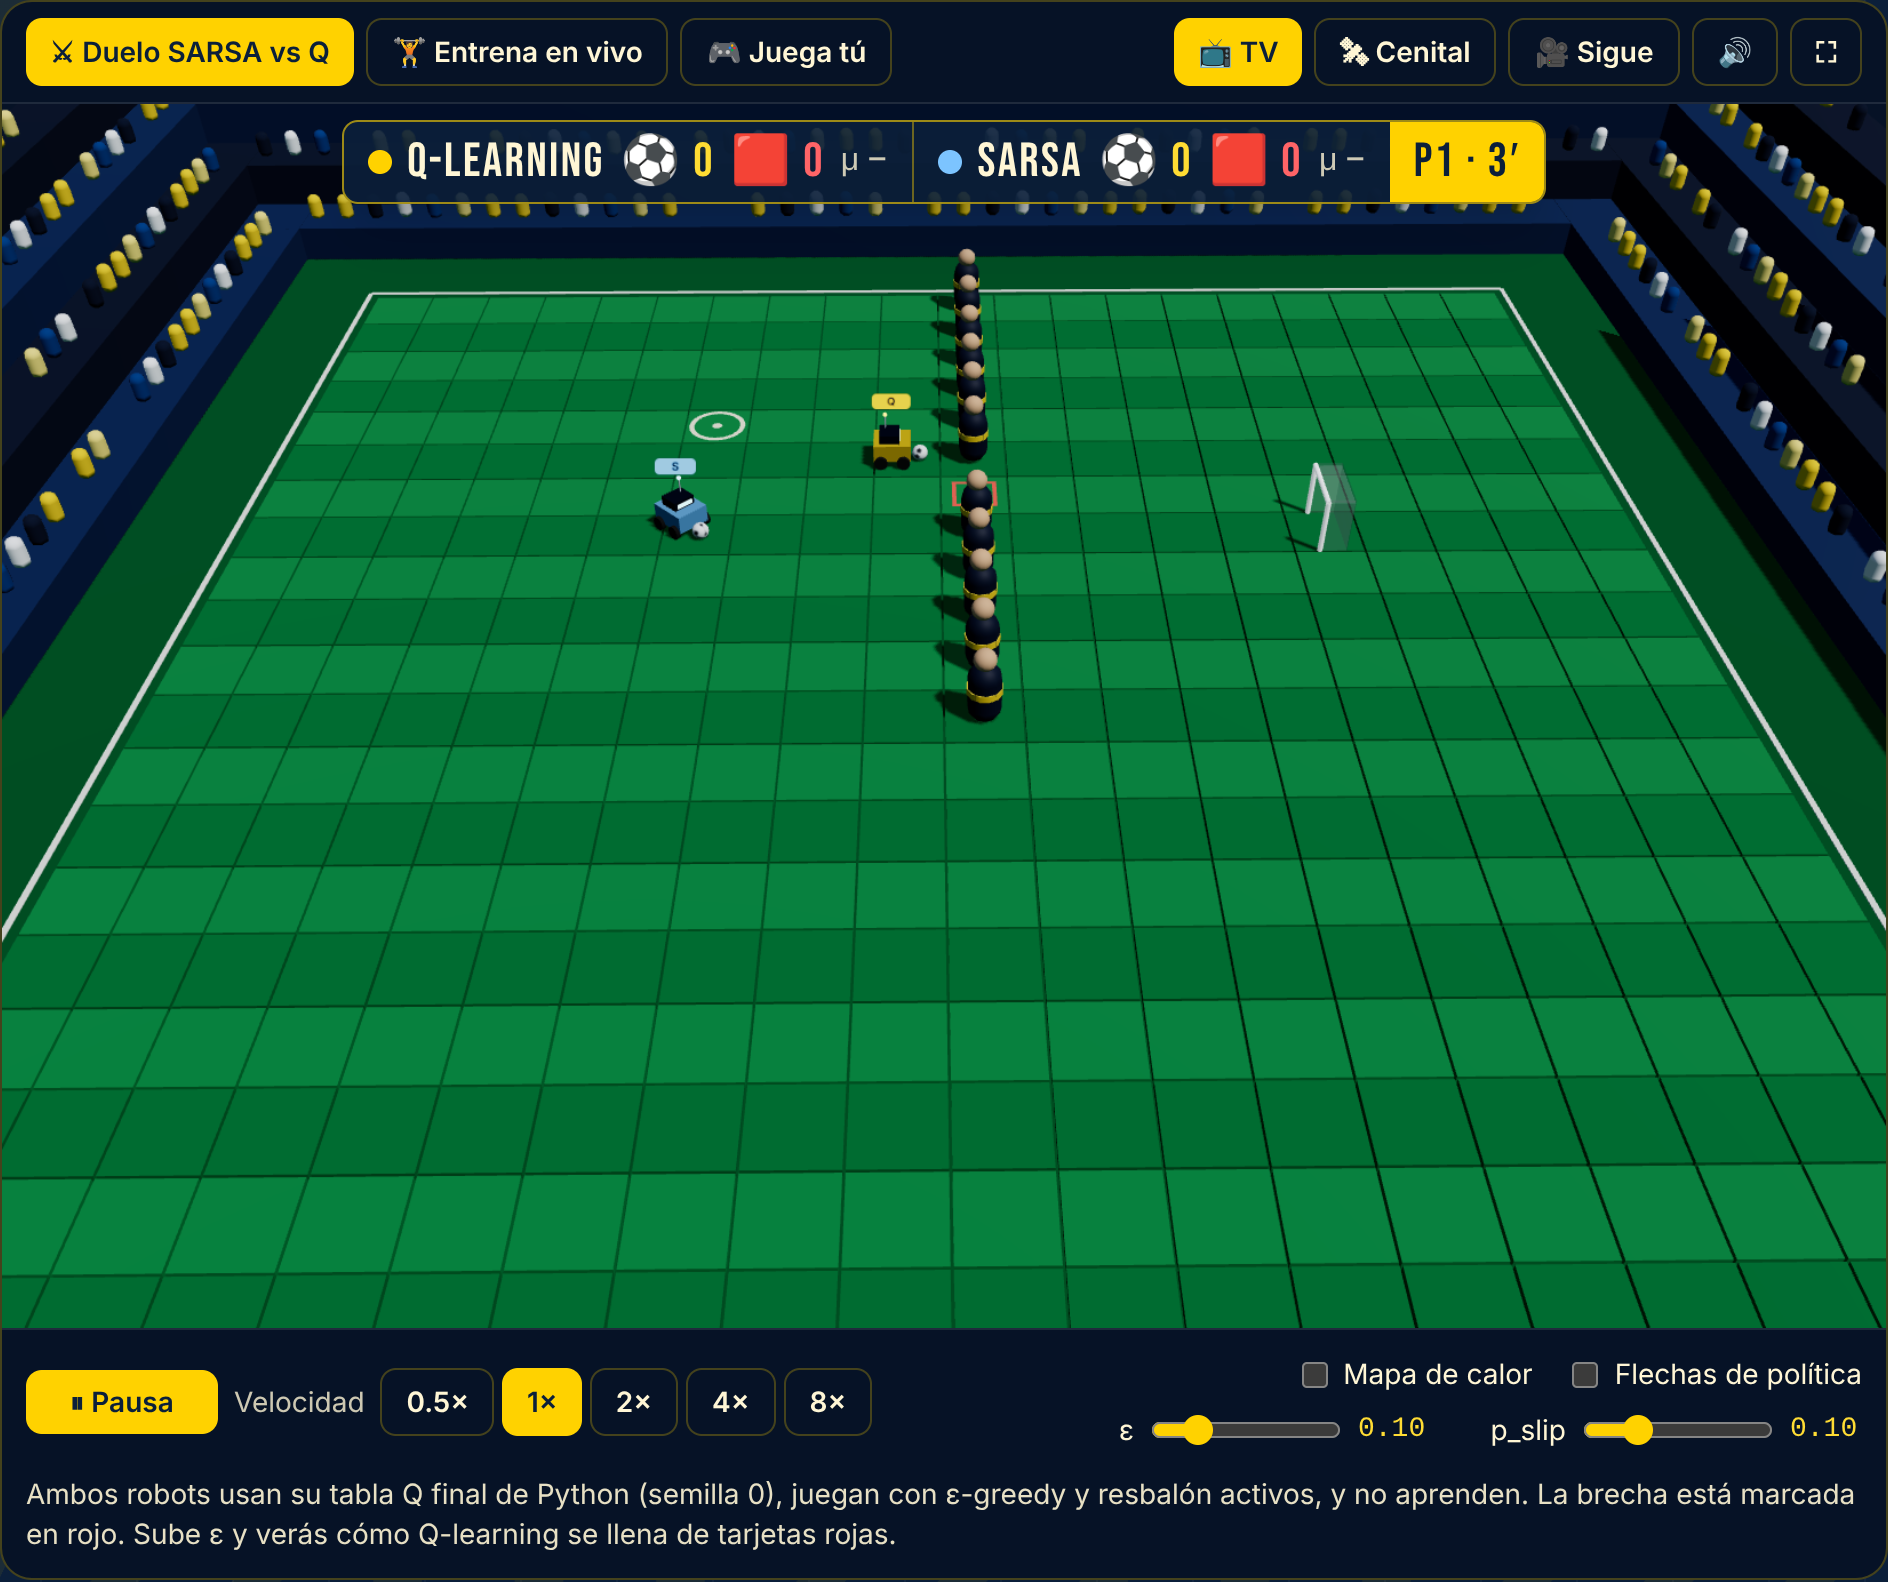
\includegraphics[width=0.75\textwidth]{images/juego_contrabandista.png}
\caption{Juego \emph{El Paso del Contrabandista 3D} en modo Duelo: Q-learning
(amarillo) se dirige a la brecha mientras SARSA (azul) baja para rodear la
barrera. El marcador muestra goles y tarjetas rojas de cada algoritmo.}
\label{fig:juego1}
\end{figure}

\begin{figure}[H]
\centering
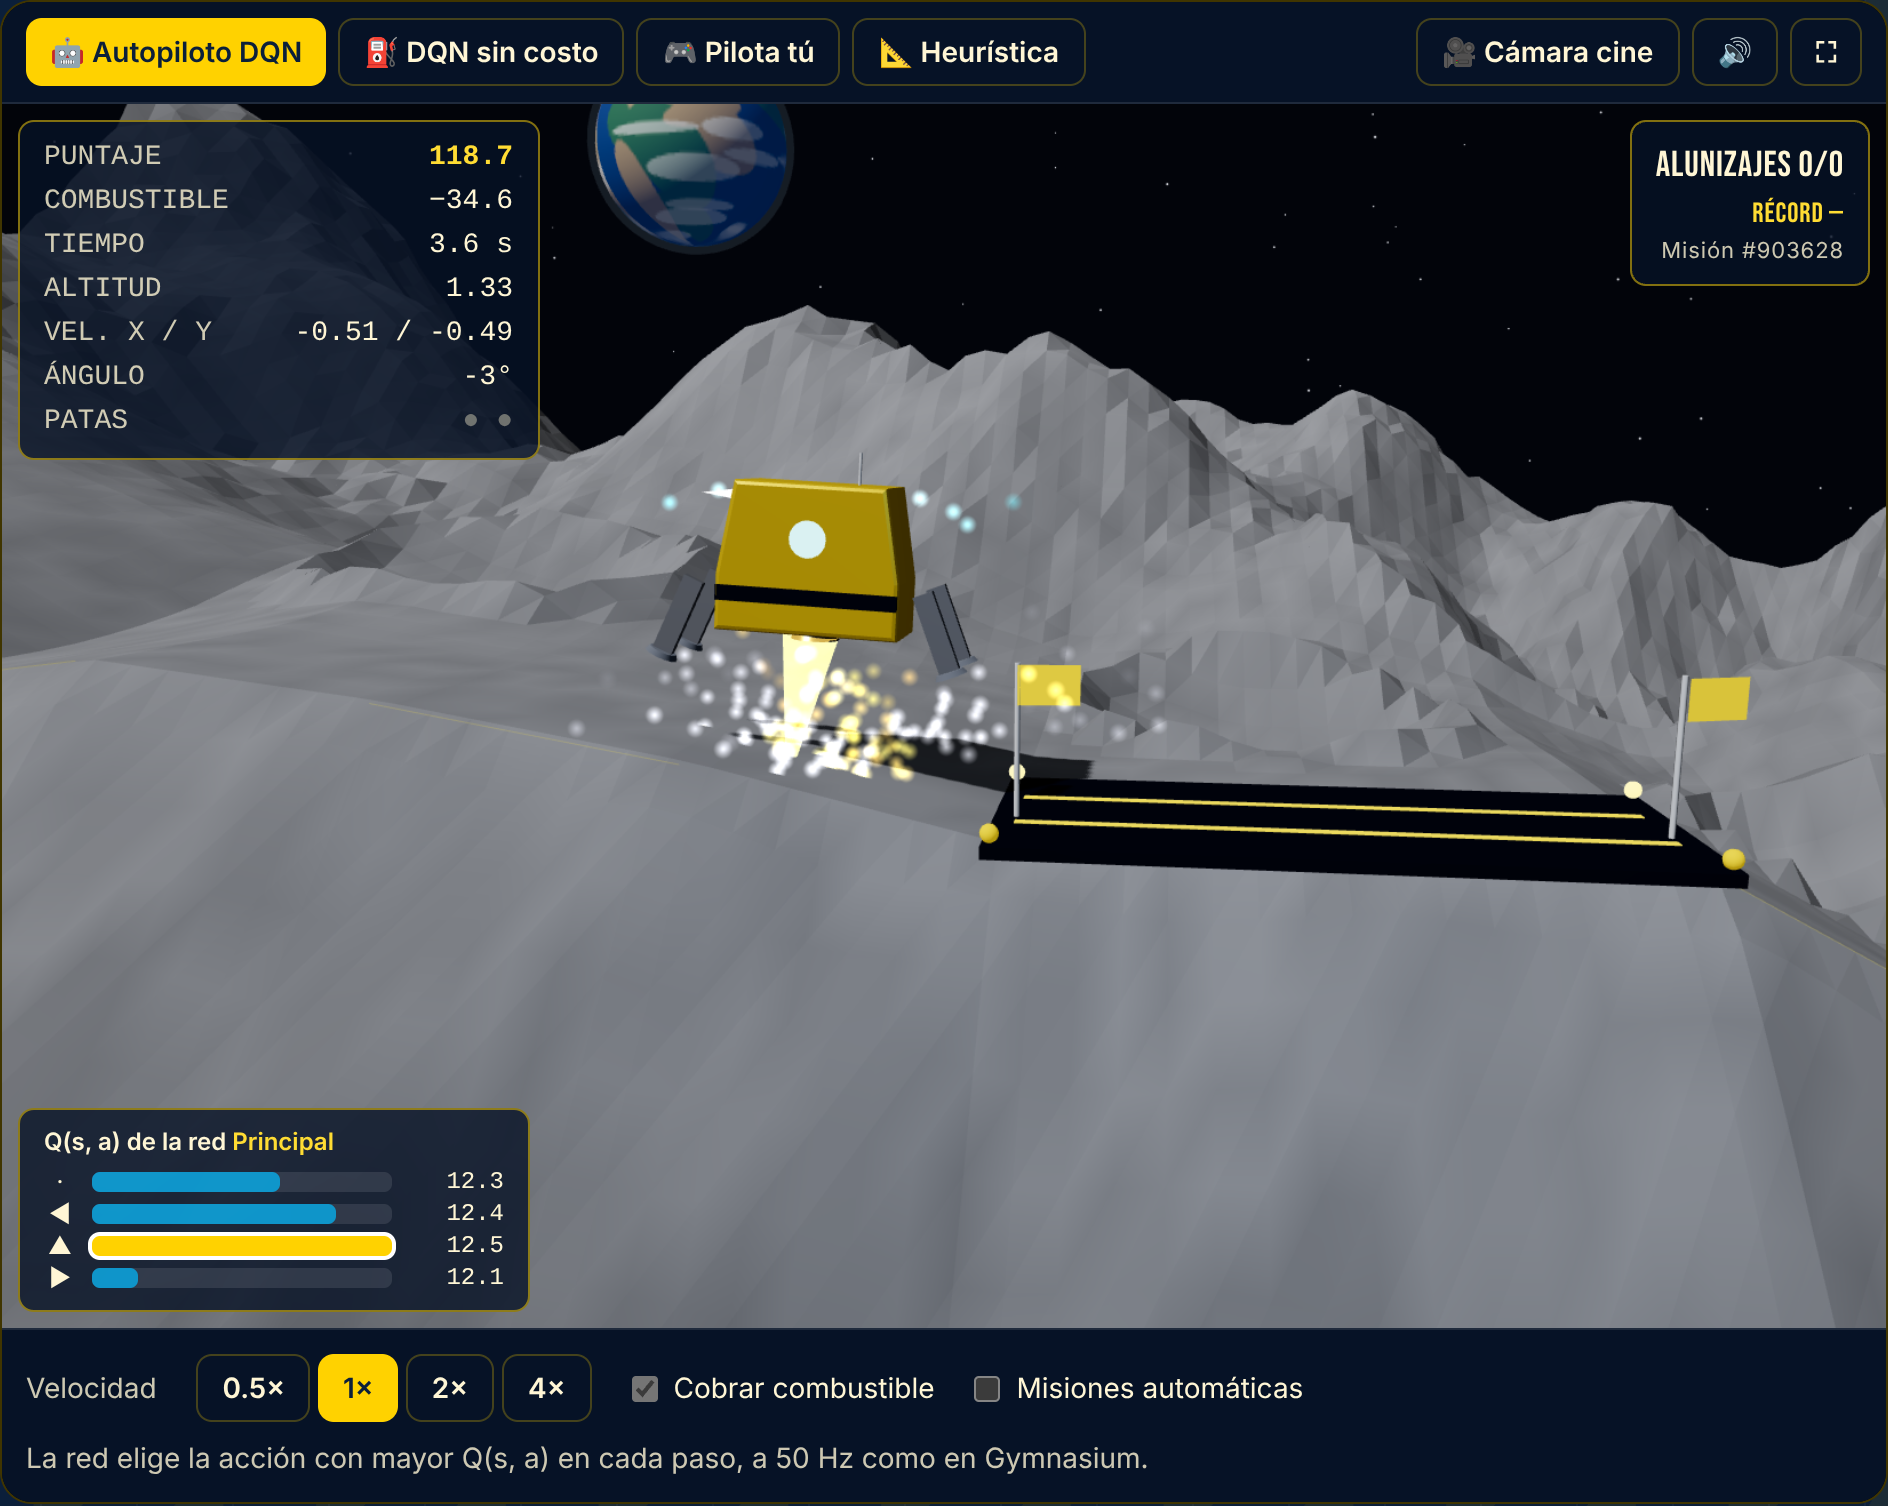
\includegraphics[width=0.49\textwidth]{images/juego_alunizaje.png}
\hfill
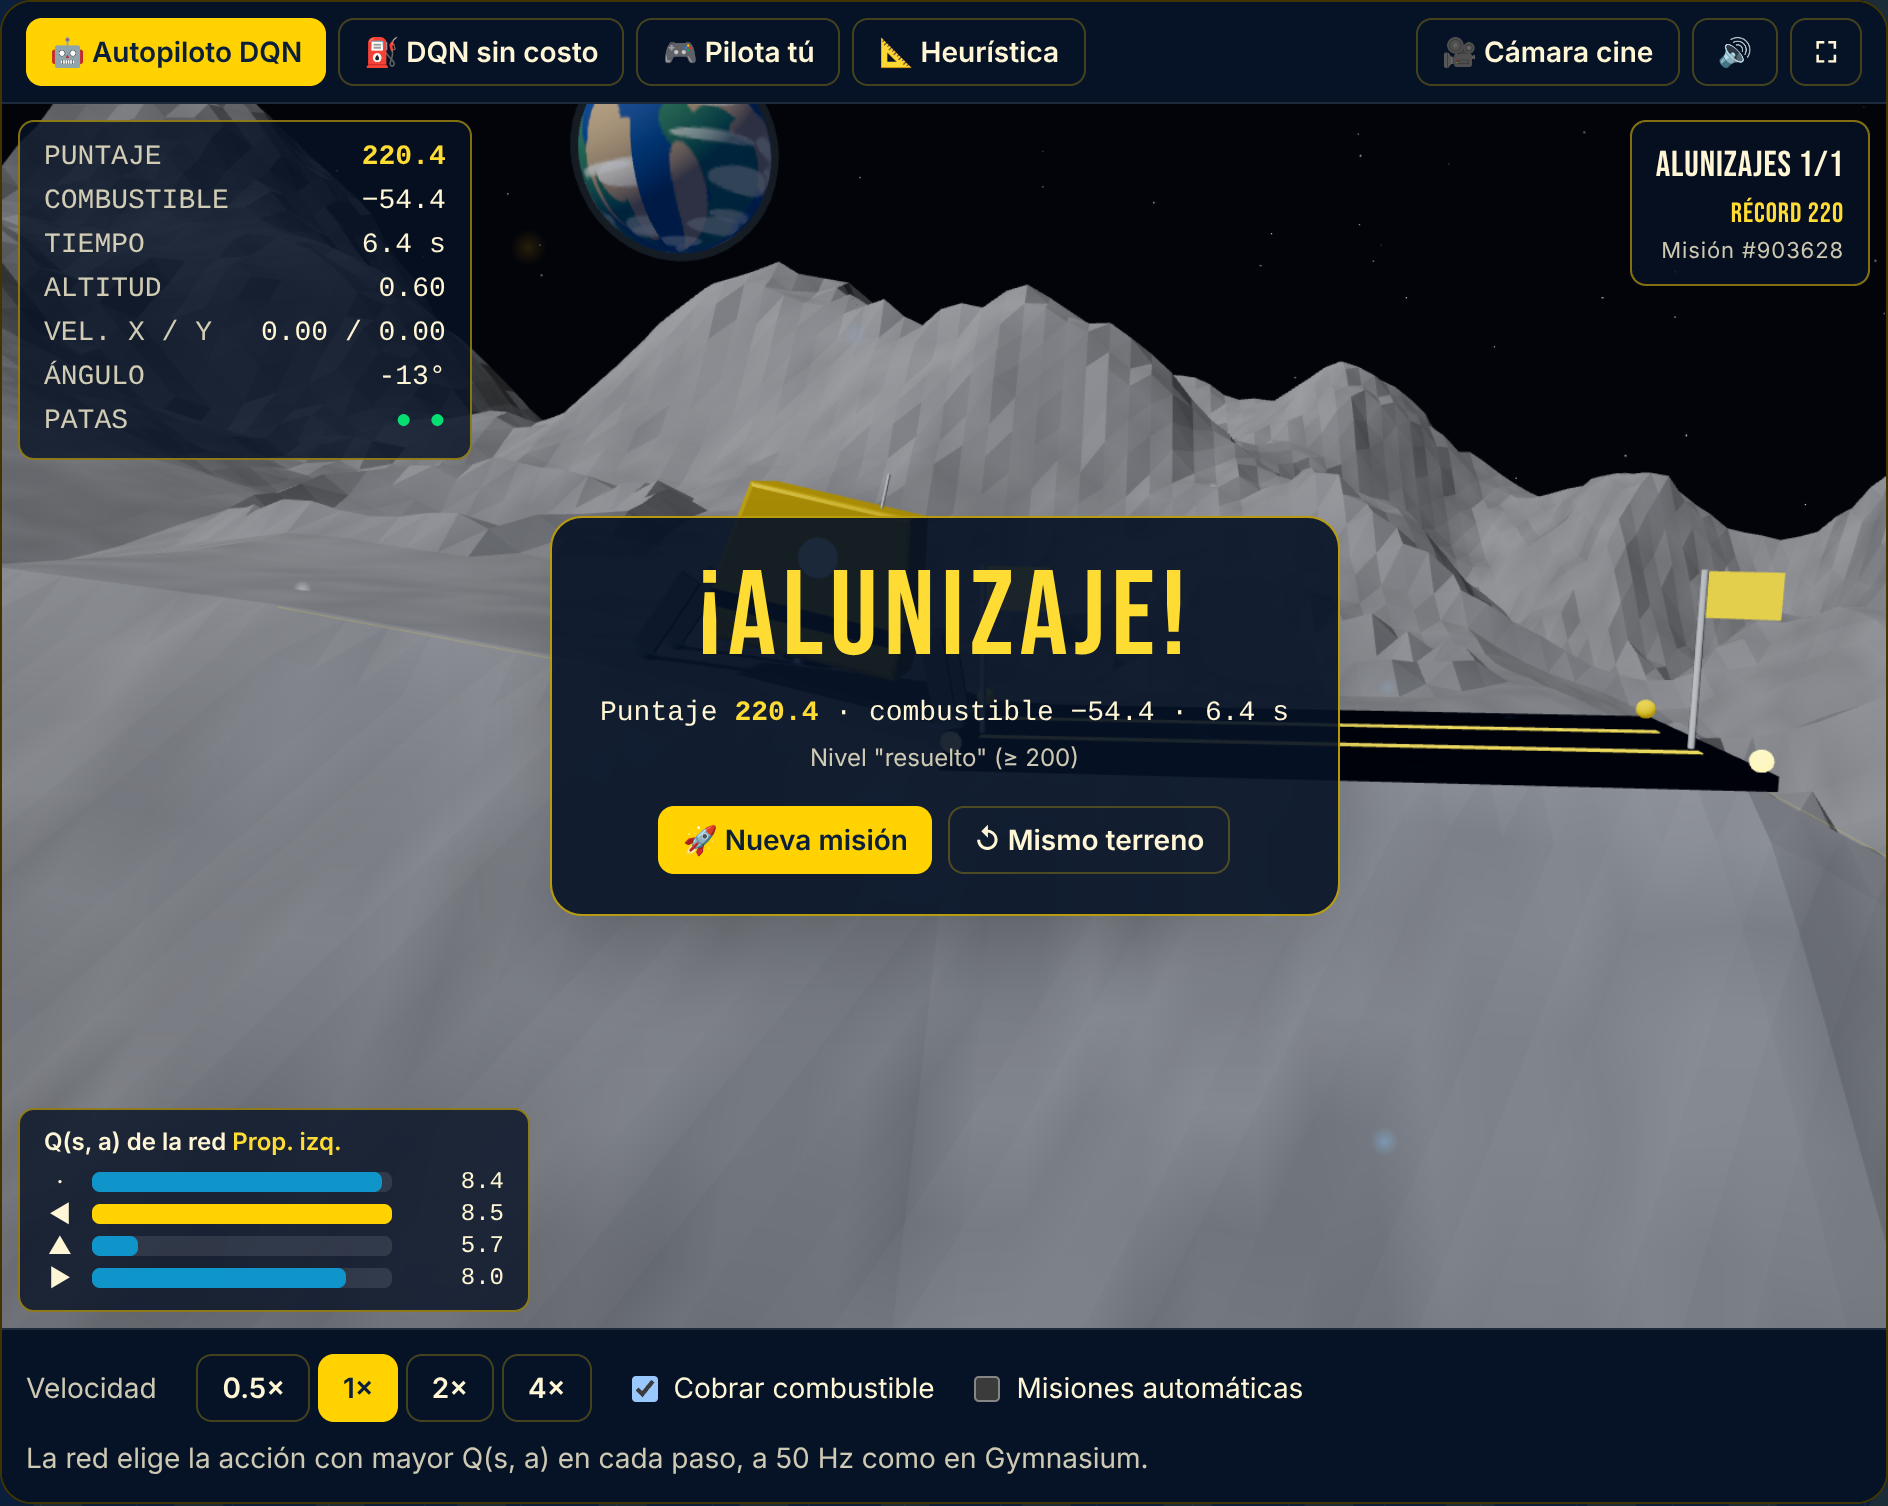
\includegraphics[width=0.49\textwidth]{images/juego_alunizaje_fin.png}
\caption{Juego \emph{Alunizaje DQN}: la red entrenada en Python pilota el módulo
en el navegador. Izquierda: motor principal encendido sobre la plataforma, con los
$Q(s,a)$ en vivo. Derecha: aterrizaje con $220.4$ puntos.}
\label{fig:juego2}
\end{figure}

\section{Resultados}

\subsection{Entregable 1: comparativa de convergencia}

Ambos agentes se entrenaron en el mismo mapa con $\alpha = 0.1$, $\gamma = 0.9$,
$\varepsilon = 0.1$ constante y $10{,}000$ episodios, repitiendo con $5$
semillas. Cada semilla es la misma para los dos algoritmos (mismo generador del
entorno y del agente). La Figura~\ref{fig:convergencia} muestra la media de las 5
semillas con una banda de $\pm 1$ desviación estándar.

\begin{figure}[H]
\centering
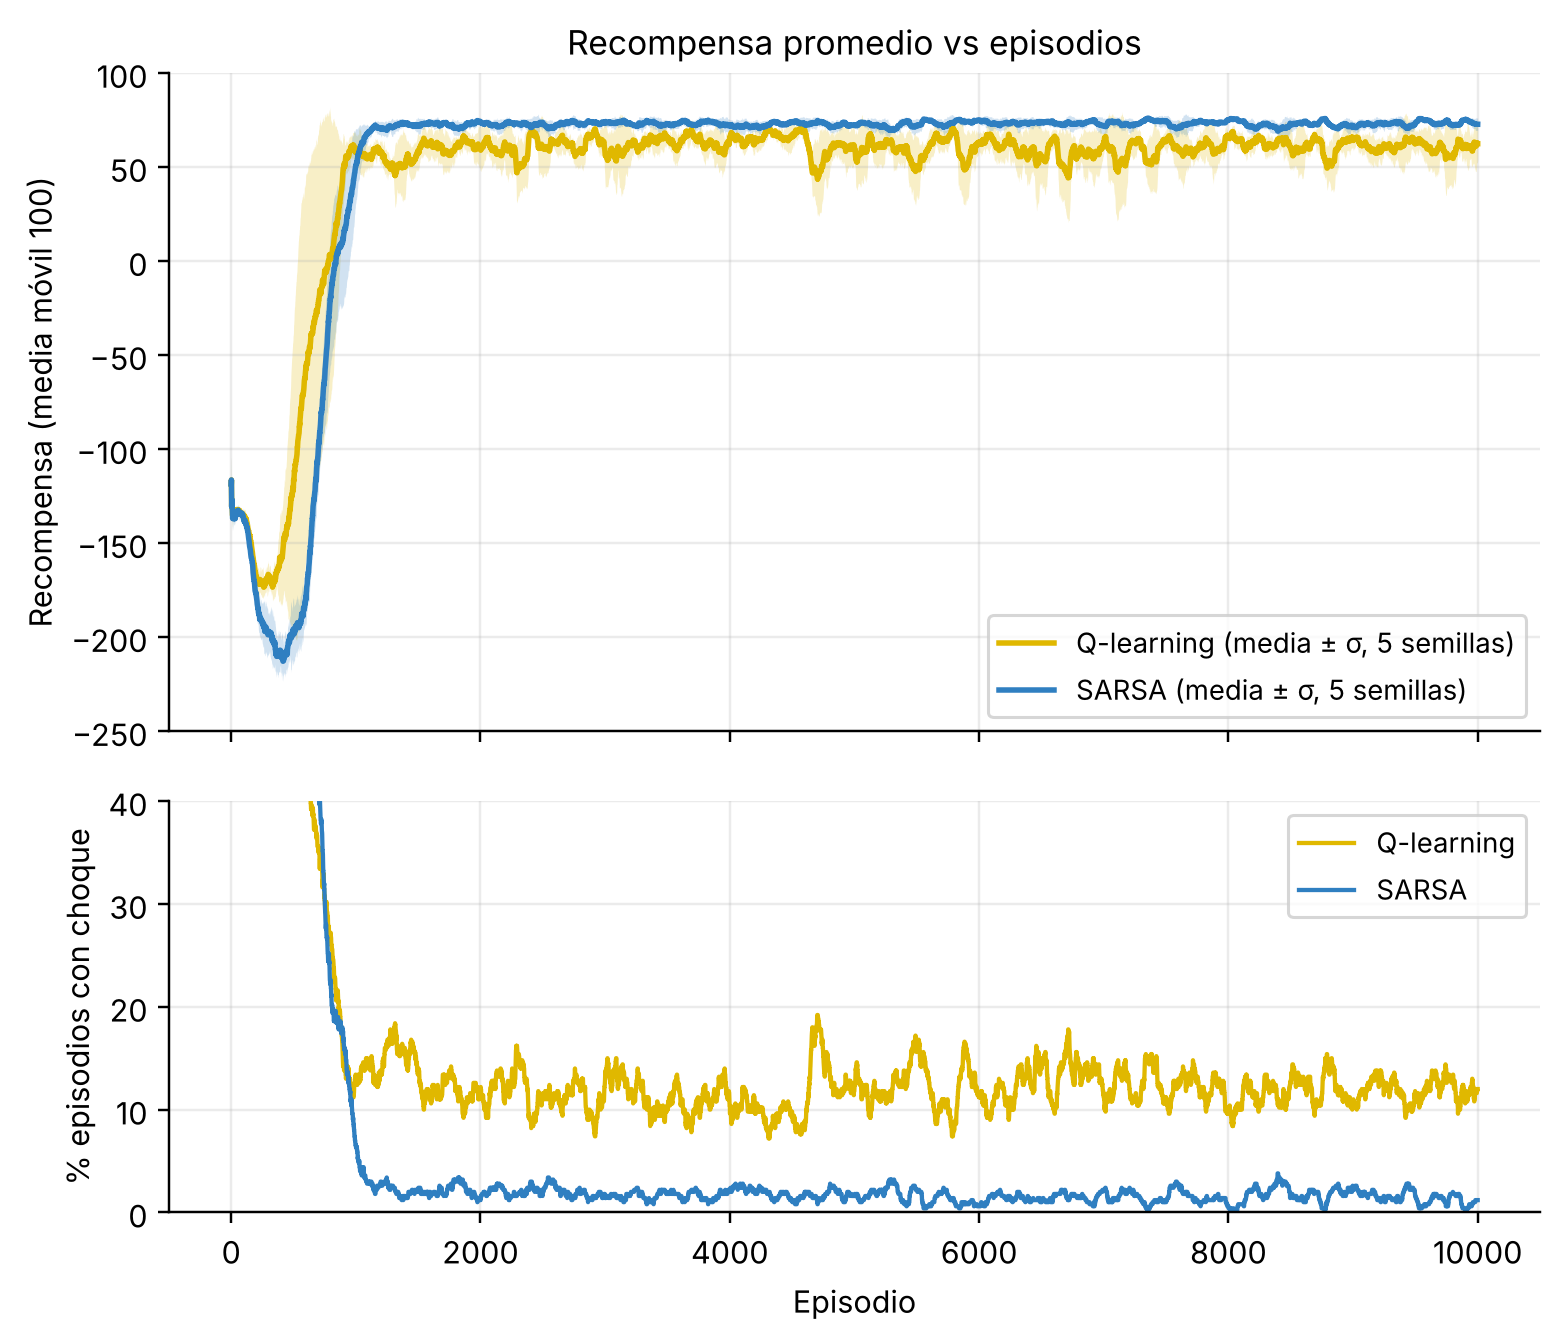
\includegraphics[width=0.85\textwidth]{images/convergencia.png}
\caption{Arriba: recompensa promedio (media móvil de 100 episodios) contra
episodios. Abajo: porcentaje de episodios que terminan en choque.}
\label{fig:convergencia}
\end{figure}

\begin{table}[H]
\centering
\renewcommand{\arraystretch}{1.2}
\begin{tabular}{|c|c|c|c|c|c|c|c|}
\hline
\rowcolor{iberoblue}
\textcolor{white}{Algoritmo} & \textcolor{white}{Sem. 0} & \textcolor{white}{Sem. 1} &
\textcolor{white}{Sem. 2} & \textcolor{white}{Sem. 3} & \textcolor{white}{Sem. 4} &
\textcolor{white}{Media $\pm$ $\sigma$} & \textcolor{white}{Choques} \\ \hline
Q-learning & $64.7$ & $53.2$ & $66.1$ & $52.6$ & $75.1$ & $62.3 \pm 8.5$ & $10.2\%$ \\ \hline
\rowcolor{yellow!30} SARSA & $76.1$ & $71.8$ & $73.0$ & $75.6$ & $66.9$ & $\mathbf{72.7 \pm 3.3}$ & $\mathbf{1.1\%}$ \\ \hline
\end{tabular}
\caption{Recompensa promedio de los últimos 100 episodios de entrenamiento por
semilla, y porcentaje de choques en la evaluación con $\varepsilon = 0.1$.}
\label{tbl:convergencia}
\end{table}

\textbf{¿Cuál converge a un valor más alto durante el entrenamiento y por qué?}
SARSA, con $72.7$ puntos por episodio contra $62.3$ de Q-learning. La razón está
en la diferencia entre (\ref{eq:qlearning}) y (\ref{eq:sarsa}):
\begin{itemize}
    \item SARSA valora cada jugada sabiendo que el $10\%$ de las veces tirará una
    acción al azar, y aprende una ruta que tolera esos errores.
    \item Q-learning aprende el valor de la política greedy óptima e ignora que él
    mismo sigue explorando. Elige la ruta corta por la brecha, donde cada acción
    aleatoria o resbalón termina en un choque de $-100$ sin el $+100$ de la meta.
\end{itemize}
Por eso la curva de Q-learning queda más abajo, es más ruidosa ($\sigma = 8.5$
contra $3.3$) y acumula unas $9$ veces más choques.

Si se apaga la exploración el resultado se invierte: con $\varepsilon = 0$, la
política de Q-learning promedia $81.1$ contra $78.9$ de SARSA, porque
Q-learning sí aprendió el camino más corto. Los primeros $\sim 1{,}500$ episodios
son muy negativos porque, con $Q = 0$ inicial, el agente deambula hasta el límite
de $400$ pasos antes de descubrir la meta.

\subsection{Entregable 2: mapas de calor de trayectorias}

La matriz de visitas cuenta cuántas veces el robot pisó cada celda una vez
entrenado. Se obtuvo en una evaluación de $1{,}000$ episodios por semilla
\textbf{con $\varepsilon = 0.1$ y resbalón activos}, sin actualizar $Q$, y se
sumaron las 5 semillas.

\textbf{¿Por qué evaluar con $\varepsilon = 0.1$ y no con la política greedy?}
Con $\varepsilon = 0$ cada agente repite casi siempre la misma trayectoria y el
riesgo de la ruta elegida casi no aparece en el mapa: no se ven los choques ni la
nube de desviaciones alrededor de la brecha. Con $\varepsilon = 0.1$ se observa
la distribución real de trayectorias, incluidos los errores, que es justo lo que
cada algoritmo valoró distinto.

\begin{figure}[H]
\centering
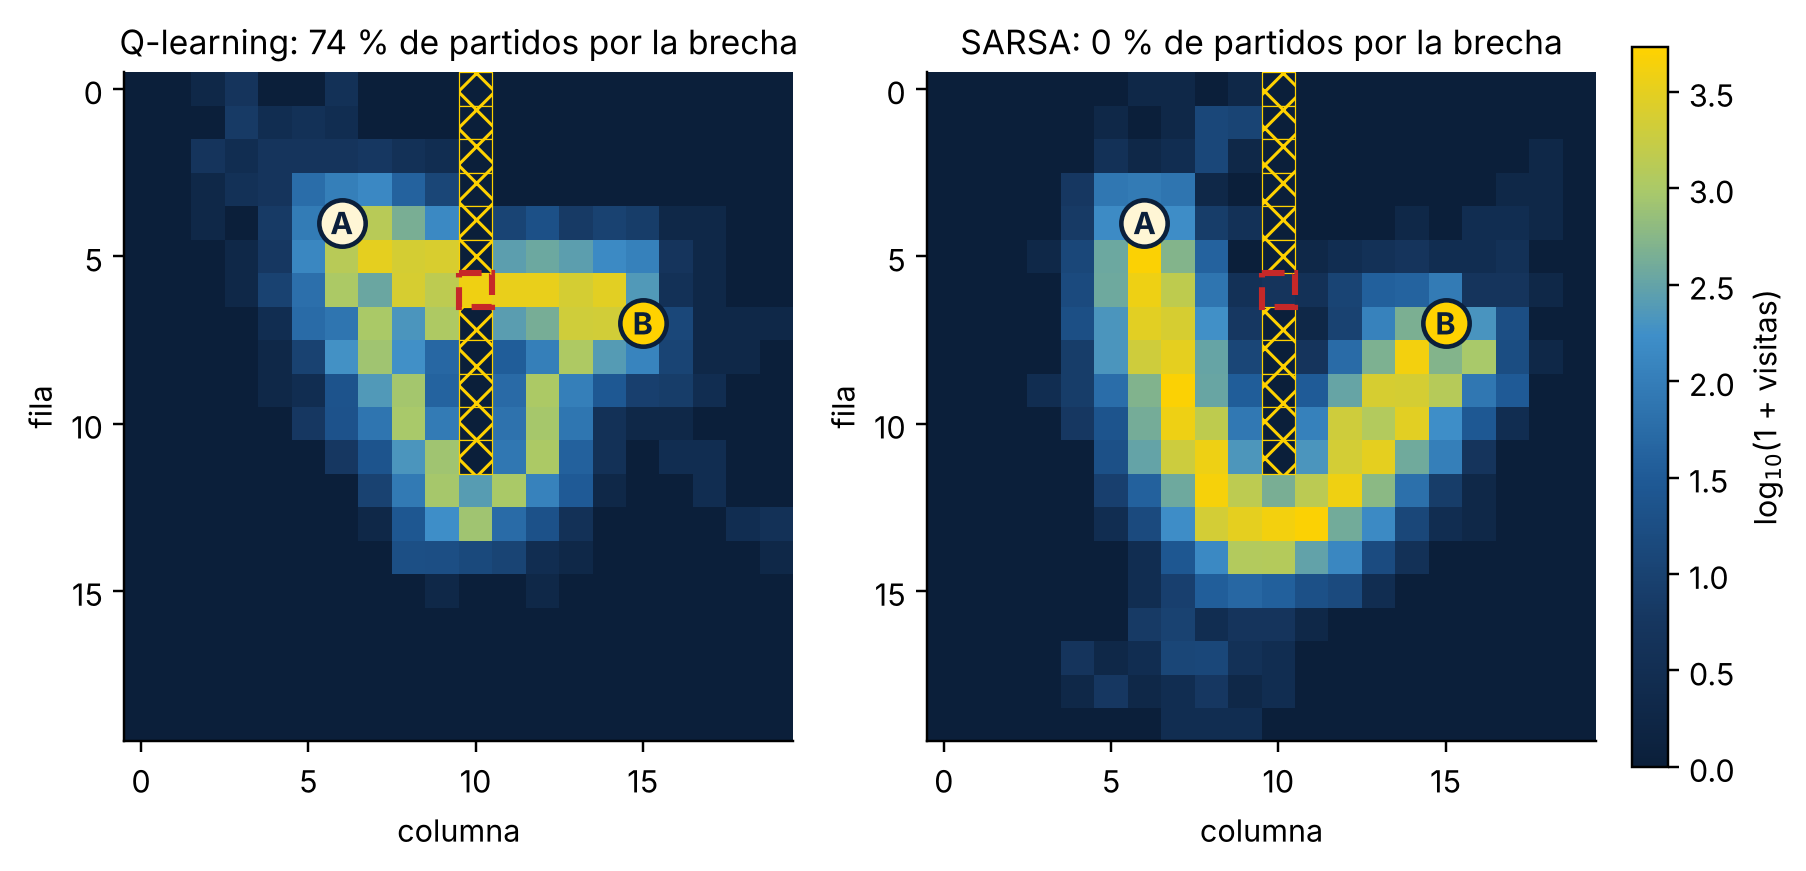
\includegraphics[width=\textwidth]{images/heatmaps.png}
\caption{Mapas de calor de visitas (escala $\log_{10}$, suma de 5 semillas) en
evaluación con $\varepsilon = 0.1$. La barrera está rayada y la brecha marcada en
rojo.}
\label{fig:heatmaps}
\end{figure}

\begin{figure}[H]
\centering
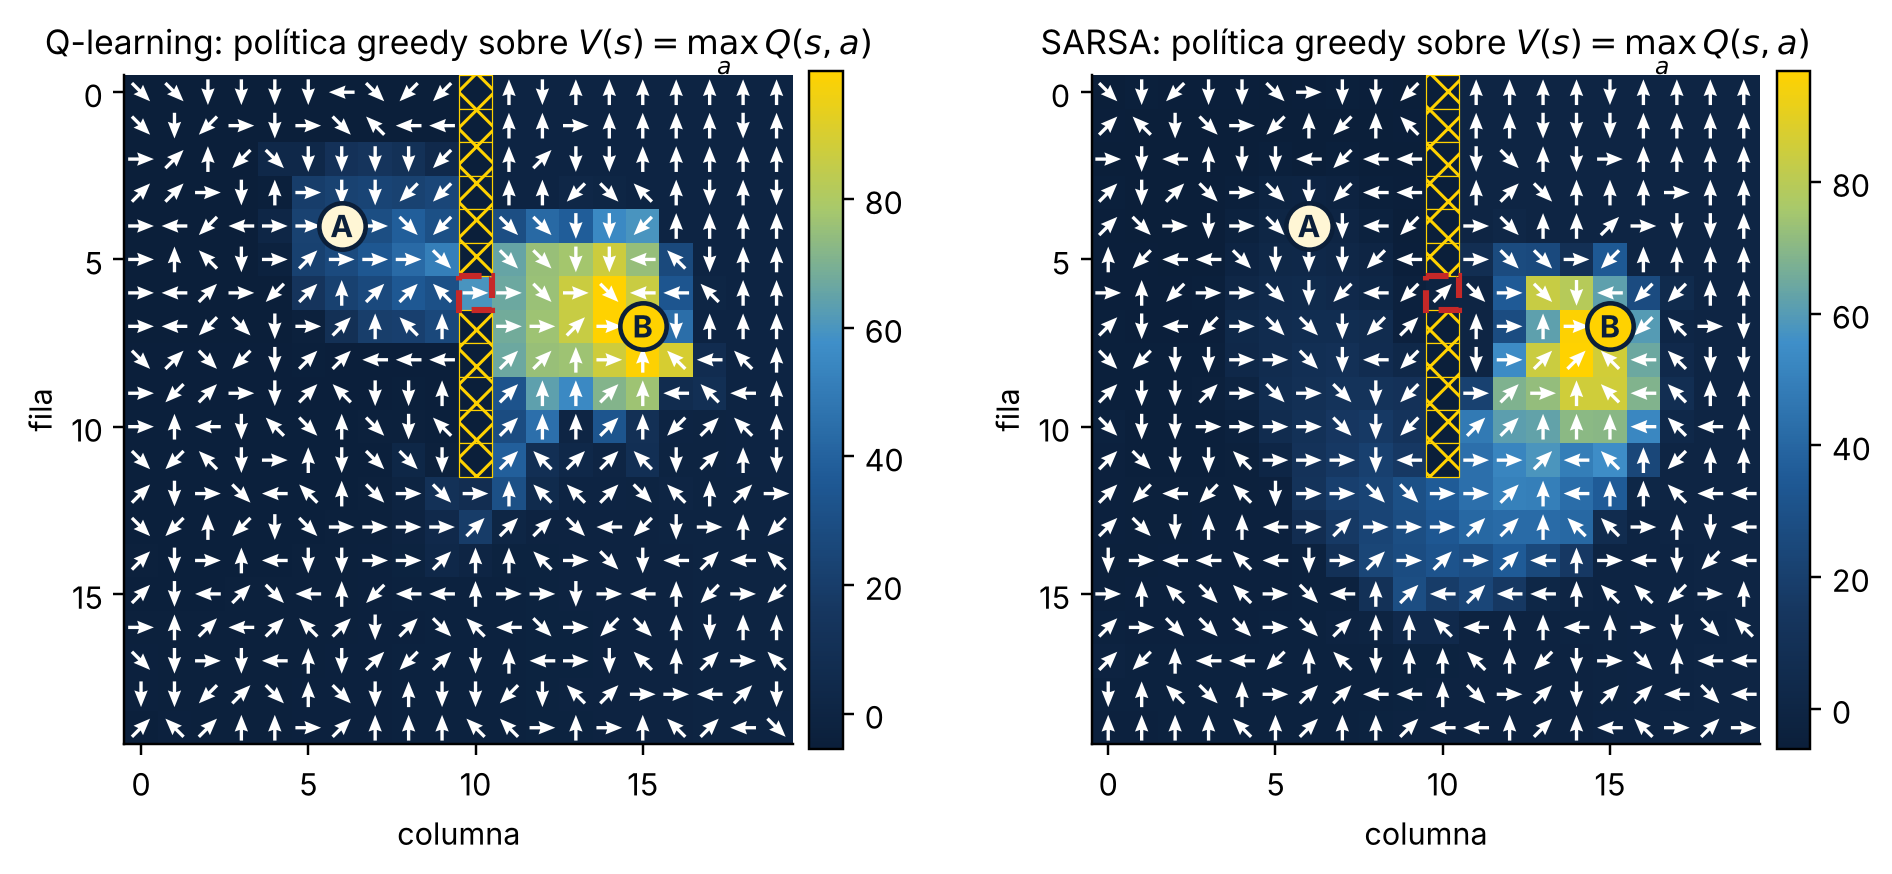
\includegraphics[width=\textwidth]{images/politicas.png}
\caption{Política greedy aprendida (flechas) sobre $V(s) = \max_a Q(s,a)$,
semilla 0. Q-learning dirige las flechas en diagonal hacia la brecha; SARSA las
desvía hacia el espacio abierto.}
\label{fig:politicas}
\end{figure}

\begin{table}[H]
\centering
\renewcommand{\arraystretch}{1.2}
\begin{tabular}{|l|c|c|c|c|}
\hline
\rowcolor{iberoblue}
\textcolor{white}{Métrica} & \textcolor{white}{Q-learning, $\varepsilon = 0.1$} &
\textcolor{white}{SARSA, $\varepsilon = 0.1$} & \textcolor{white}{Q-learning, $\varepsilon = 0$} &
\textcolor{white}{SARSA, $\varepsilon = 0$} \\ \hline
Recompensa media   & $65.7$   & $\mathbf{73.4}$ & $\mathbf{81.1}$ & $78.9$ \\ \hline
Llega a la meta    & $89.8\%$ & $98.9\%$        & $96.7\%$        & $100\%$ \\ \hline
Choques            & $10.2\%$ & $1.1\%$         & $3.3\%$         & $0\%$ \\ \hline
Usa la brecha      & $74\%$   & $0.1\%$         & $77\%$          & $0\%$ \\ \hline
Pasos por episodio & $12.6$   & $21.6$          & $11.2$          & $18.8$ \\ \hline
\end{tabular}
\caption{Evaluación sin aprendizaje: $1{,}000$ episodios por semilla, promedio de
las 5 semillas.}
\label{tbl:evaluacion}
\end{table}

\textbf{Hipótesis verificada.}
\begin{itemize}
    \item \textbf{Q-learning corta esquinas:} el $74\%$ de sus episodios pasa por
    la brecha de una celda, rozando las esquinas de la barrera. En cuatro de las
    cinco semillas su política greedy usa la brecha; en la semilla 2 nunca la
    descubrió con $\varepsilon$ constante y se quedó con la ruta larga.
    \item \textbf{SARSA mantiene un colchón de seguridad:} prácticamente nunca usa
    la brecha ($0.1\%$). Rodea la barrera por abajo, sin pegarse a su punta, y se
    mantiene lejos de las paredes exteriores. Su $V(s)$ en la brecha es mucho más
    bajo porque ahí la exploración se paga con tarjeta roja.
\end{itemize}

\subsection{Entregable 3: discusión sobre robótica real}

En un robot físico costoso que comparte espacio con personas se elegiría
\textbf{SARSA}, o en general un método on-policy y conservador. En el mundo real
el robot nunca deja de tener ruido: patina, los sensores fallan y, mientras
aprende o se adapta, sigue explorando. Q-learning optimiza el valor de una
política ideal que supone que nunca se equivoca, lo que produce rutas pegadas a
las esquinas donde un solo error cuesta un choque; aquí ese choque vale $-100$,
pero en la realidad es un robot roto o una persona lastimada. SARSA incorpora en
$Q(s',a')$ la probabilidad real de equivocarse y por eso es \textbf{aversa al
riesgo} (\emph{risk averse}): sacrifica un poco de recompensa esperada (una ruta
más larga) a cambio de reducir mucho la varianza y la probabilidad de un
desenlace catastrófico. En nuestros datos eso se tradujo en unas $9$ veces menos
choques con $\varepsilon = 0.1$. En robótica de servicio el costo de un fallo es
asimétrico e irreversible, así que ese colchón vale más que unos pasos ahorrados.
Si se usara Q-learning, convendría apagar la exploración al desplegar y añadir
restricciones de seguridad explícitas, como zonas prohibidas, márgenes o
penalizaciones de proximidad.

\subsection{Entregable DQN 1: curva de aprendizaje}

La red se entrenó en CPU durante $128$~s con la semilla 0 y se detuvo en el
\textbf{episodio 526}, cuando la media móvil de 100 episodios superó $+200$
(con $\varepsilon$ ya en $0.072$). La Figura~\ref{fig:dqn} muestra la recompensa
por episodio, la media móvil y $\varepsilon$, con las fases del aprendizaje
detectadas automáticamente en los datos (Tabla~\ref{tbl:fases}).

\begin{figure}[H]
\centering
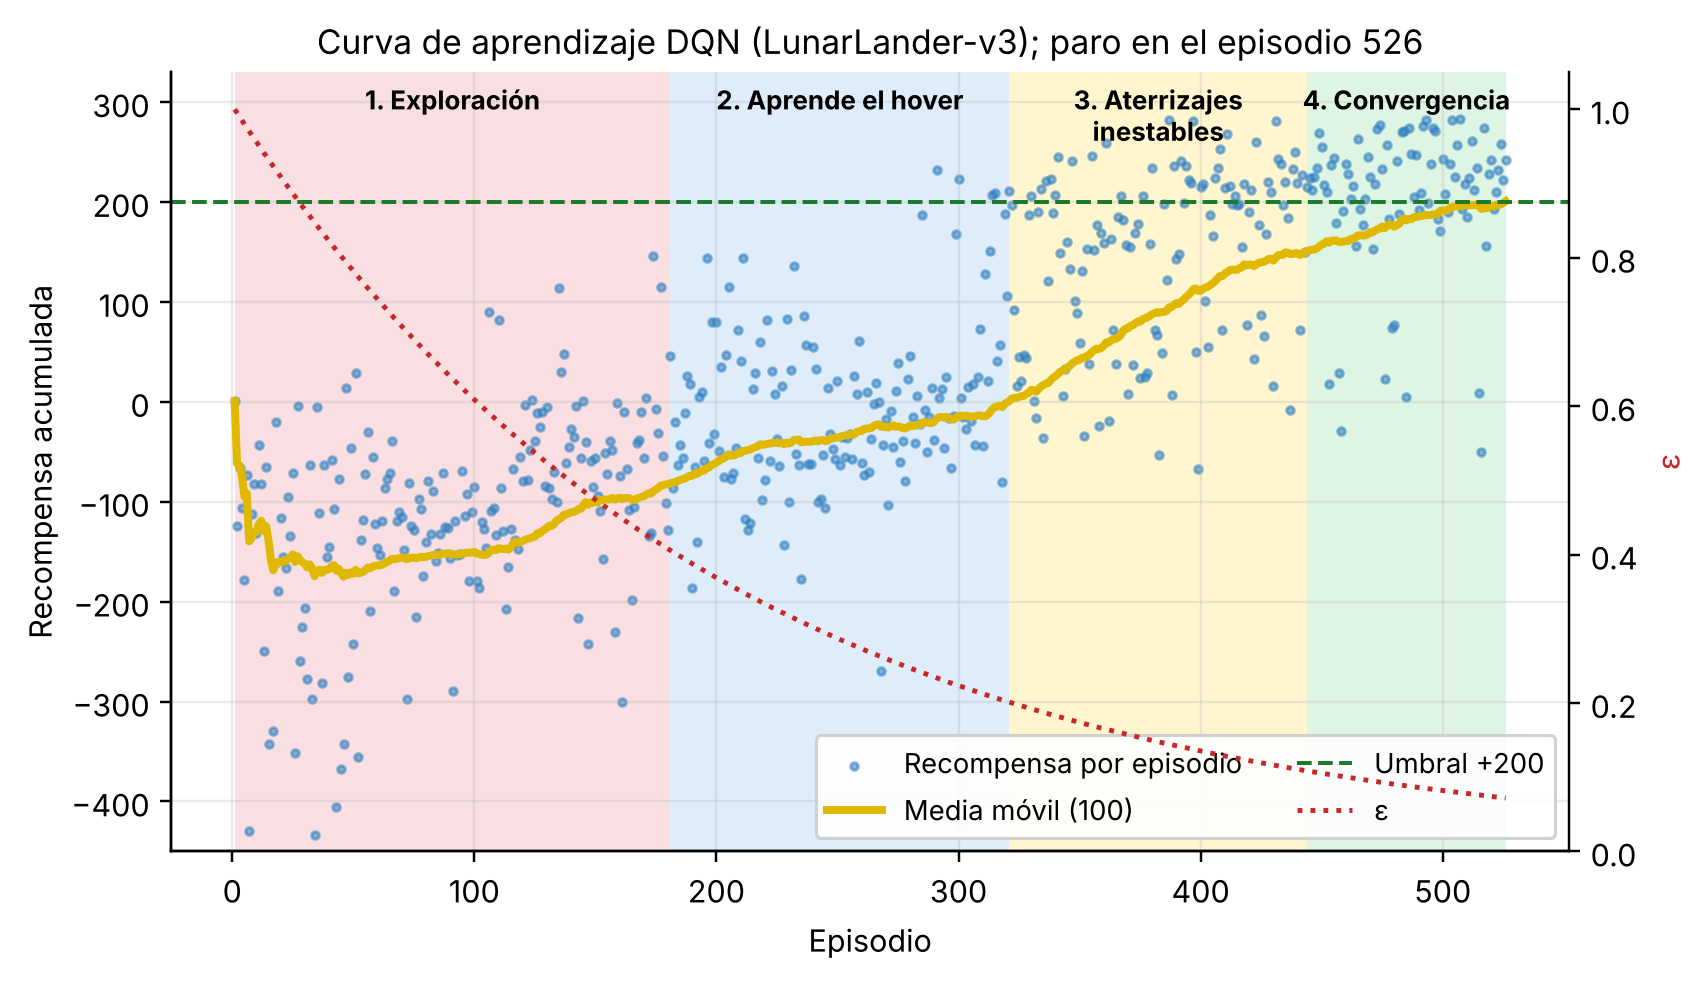
\includegraphics[width=0.92\textwidth]{images/dqn_curva.png}
\caption{Curva de aprendizaje de DQN con las cuatro fases sombreadas.}
\label{fig:dqn}
\end{figure}

\begin{table}[H]
\centering
\renewcommand{\arraystretch}{1.2}
\begin{tabular}{|c|c|p{9.3cm}|}
\hline
\rowcolor{iberoblue}
\textcolor{white}{Fase} & \textcolor{white}{Episodios} & \textcolor{white}{Comportamiento observado} \\ \hline
1. Exploración & $1$--$181$ & $\varepsilon$ alto: acciones casi aleatorias; el módulo choca en $\sim 100$ pasos y la media ronda $-150$. \\ \hline
2. Aprende el \emph{hover} & $181$--$321$ & Descubre que flotar evita el $-100$: hasta el $86\%$ de los episodios llega al límite de $1{,}000$ pasos. Inicia cuando $\ge 10\%$ de los últimos 50 episodios agotan el tiempo. \\ \hline
3. Aterrizajes inestables & $321$--$444$ & Empieza a posarse (de $8\%$ a $80\%$ de aterrizajes), a veces rebota o se inclina. Inicia cuando $\ge 20\%$ de los últimos 50 episodios aterrizan. \\ \hline
4. Convergencia & $444$--$526$ & Aterrizajes consistentes entre las banderas; la media móvil pasa de $150$ a $+200$. \\ \hline
\end{tabular}
\caption{Fases del aprendizaje del DQN.}
\label{tbl:fases}
\end{table}

\begin{figure}[H]
\centering
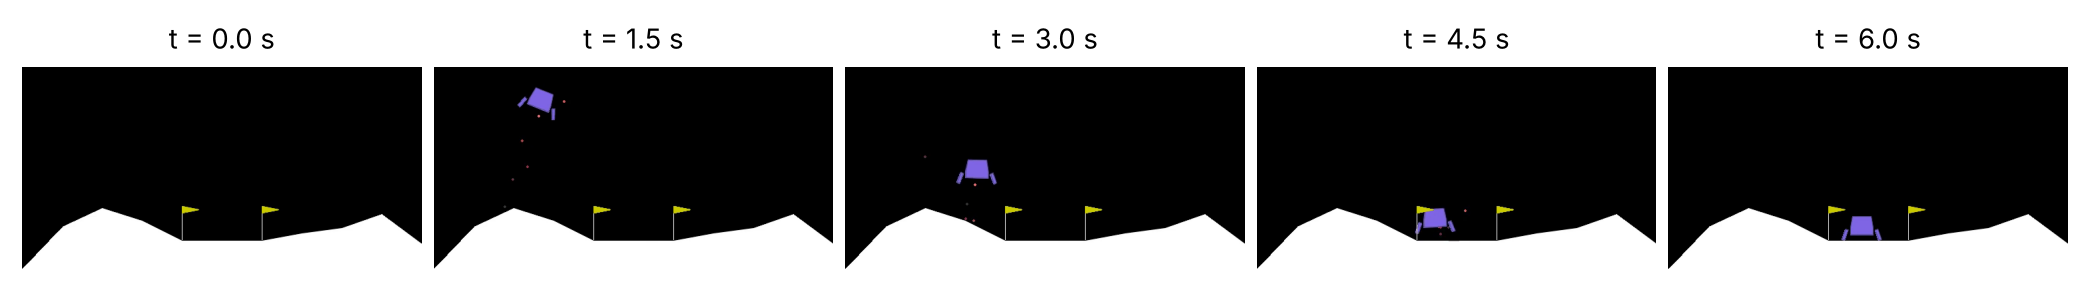
\includegraphics[width=\textwidth]{images/aterrizaje.png}
\caption{Aterrizaje con la política greedy final en Gymnasium (recompensa $294.3$).}
\label{fig:aterrizaje}
\end{figure}

La evaluación greedy ($\varepsilon = 0$) en 20 episodios dio $\mathbf{160.9 \pm 79.6}$,
con $55\%$ de aterrizajes. Queda por debajo de 200 aunque la media de
entrenamiento lo superó: al parar justo en el umbral, el agente conserva algo del
hábito de la fase 2, y $7$ de los $20$ episodios greedy se quedan flotando hasta
los $1{,}000$ pasos. Durante el entrenamiento el $\varepsilon$ restante lo sacaba
del \emph{hover}; con $\varepsilon = 0$ no hay nada que lo empuje. Para comprobar
que no es un efecto de la semilla se repitió el entrenamiento completo con cuatro
semillas (Tabla~\ref{tbl:semillas}). Con $100$ episodios de evaluación, la red de
la semilla 0 obtiene $193.3 \pm 59.5$ y $77\%$ de aterrizajes
(Tabla~\ref{tbl:validacion}).

\begin{table}[H]
\centering
\renewcommand{\arraystretch}{1.2}
\begin{tabular}{|c|c|c|c|c|}
\hline
\rowcolor{iberoblue}
\textcolor{white}{Semilla} & \textcolor{white}{Paro (media $\ge 200$)} &
\textcolor{white}{Greedy, media $\pm$ $\sigma$} & \textcolor{white}{Aterrizajes} &
\textcolor{white}{Se queda flotando} \\ \hline
$0$ & episodio $526$ & $160.9 \pm 79.6$ & $55\%$ & $7/20$ \\ \hline
$1$ & episodio $500$ & $196.5 \pm 89.3$ & $90\%$ & $1/20$ \\ \hline
$2$ & episodio $570$ & $215.7 \pm 44.3$ & $90\%$ & $2/20$ \\ \hline
$3$ & episodio $478$ & $199.7 \pm 75.2$ & $85\%$ & $2/20$ \\ \hline
\textbf{Promedio} & \textbf{episodio 519} & $\mathbf{193.2}$ & $\mathbf{80\%}$ & --- \\ \hline
\end{tabular}
\caption{Repetición del entrenamiento DQN con cuatro semillas (evaluación greedy
de 20 episodios).}
\label{tbl:semillas}
\end{table}

\subsection{Entregable DQN 2: análisis de la función de recompensa}

La recompensa resta $0.3$ por cada cuadro con el motor principal y $0.03$ por cada
cuadro con un propulsor lateral. Un aterrizaje enciende el motor cientos de
veces, de modo que este término suma decenas de puntos y \textbf{define el estilo
de vuelo}:
\begin{itemize}
    \item \textbf{Con penalización}, la política óptima es eficiente: deja caer el
    módulo casi en caída libre, frena con ráfagas cortas y tardías del motor
    principal, corrige el ángulo con los propulsores laterales (diez veces más
    baratos) y apaga todo en cuanto las patas tocan el suelo.
    \item \textbf{Con costo cero}, encender motores es gratis y emerge el
    \emph{hover} prolongado: mantenerse suspendido es una forma segura de evitar el
    $-100$ y no cuesta nada. El agente usa el motor principal de más, desciende
    lento y tarda en asentarse; con $\gamma = 0.99$ hay poco apuro por cobrar el
    $+100$ pronto. En un sistema real eso significa combustible desperdiciado y
    menos autonomía.
\end{itemize}

Para comprobarlo se entrenó una variante con un \emph{wrapper} que devuelve la
penalización de combustible, con el mismo código, hiperparámetros y semilla.

\begin{table}[H]
\centering
\renewcommand{\arraystretch}{1.2}
\begin{tabular}{|l|c|c|}
\hline
\rowcolor{iberoblue}
\textcolor{white}{Política greedy, 20 episodios} & \textcolor{white}{Con costo (original)} &
\textcolor{white}{Costo $= 0$} \\ \hline
Encendidos del motor principal por episodio & $175$ & $\mathbf{350}$ \\ \hline
Encendidos de propulsores laterales         & $324$ & $217$ \\ \hline
Duración media (pasos)                      & $631$ & $691$ \\ \hline
Episodios que agotan los $1{,}000$ pasos    & $7/20$ & $4/20$ \\ \hline
Aterrizajes                                 & $55\%$ & $75\%$ \\ \hline
Recompensa que optimiza                     & $160.9 \pm 79.6$ & $239.4 \pm 62.2$ \\ \hline
Recompensa original (con combustible)       & $160.9 \pm 79.6$ & $128.1 \pm 80.5$ \\ \hline
Episodio en que la media móvil llega a $200$ & $526$ & $404$ \\ \hline
\end{tabular}
\caption{Efecto de la penalización por combustible.}
\label{tbl:combustible}
\end{table}

\begin{figure}[H]
\centering
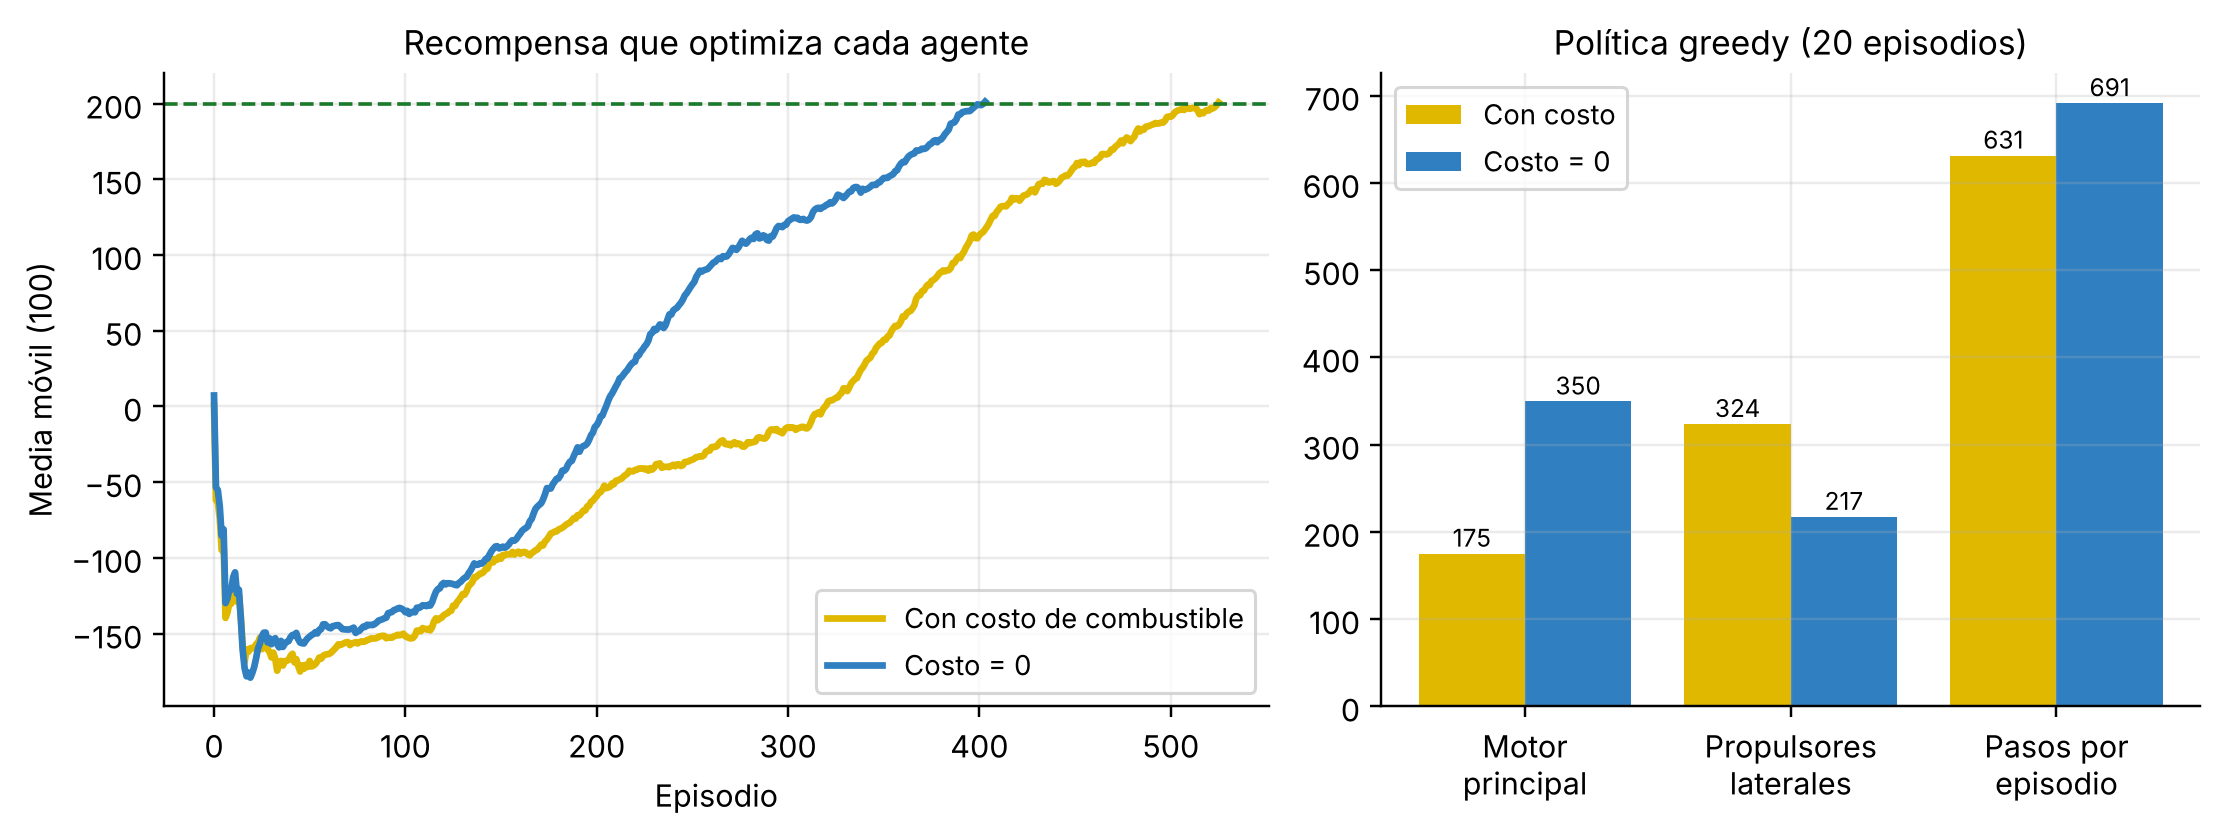
\includegraphics[width=\textwidth]{images/combustible.png}
\caption{Izquierda: media móvil de la recompensa que optimiza cada agente.
Derecha: uso de motores y duración de los episodios con la política greedy.}
\label{fig:combustible}
\end{figure}

Sin costo, el agente enciende el motor principal el \textbf{doble} de veces y sus
episodios duran un $10\%$ más. Su puntaje ``inflado'' de $239.4$ se desploma a
$128.1$ cuando se le cobra la gasolina. Además alcanza el umbral antes (episodio
$404$ contra $526$): el problema es más fácil porque explorar con los motores no
se castiga, pero la política resultante es derrochadora. Como matiz, en esta
corrida el agente \emph{con} costo se queda flotando más veces ($7/20$ contra
$4/20$) porque se detuvo justo en el umbral; la diferencia de estilo se ve en
cuánto empuja, no en si termina el episodio.

\subsection{Entregable DQN 3: escalabilidad tabular frente a redes profundas}

Si cada variable continua del módulo se discretiza en 20 segmentos:
\begin{align*}
\text{Las 8 variables:}\quad & |\mathcal{S}| = 20^8 = 2.56 \times 10^{10} \text{ estados},\quad
|\mathcal{S}| \cdot |\mathcal{A}| = 2.56 \times 10^{10} \times 4 = 1.024 \times 10^{11} \text{ entradas},\\
& 1.024 \times 10^{11} \times 4\,\text{B} = 4.10 \times 10^{11}\,\text{B} \approx 410\ \text{GB}.\\[4pt]
\text{Patas binarias:}\quad & |\mathcal{S}| = 20^6 \times 2^2 = 2.56 \times 10^{8} \text{ estados},\quad
2.56 \times 10^{8} \times 4 = 1.024 \times 10^{9} \text{ entradas},\\
& 1.024 \times 10^{9} \times 4\,\text{B} = 4.10 \times 10^{9}\,\text{B} \approx 4.1\ \text{GB}.\\[4pt]
\text{Red neuronal:}\quad & 18{,}180 \text{ parámetros} \times 4\,\text{B} = 72{,}720\,\text{B} \approx 72.7\ \text{KB}.
\end{align*}

\begin{table}[H]
\centering
\renewcommand{\arraystretch}{1.2}
\begin{tabular}{|l|c|c|c|}
\hline
\rowcolor{iberoblue}
\textcolor{white}{Representación} & \textcolor{white}{Entradas / parámetros} &
\textcolor{white}{Memoria (float32)} & \textcolor{white}{Veces la red} \\ \hline
Tabla Q, 8 variables $\times$ 20 & $1.024 \times 10^{11}$ & $\approx 410$ GB & $\approx 5.6 \times 10^{6}$ \\ \hline
Tabla Q, patas binarias          & $1.024 \times 10^{9}$  & $\approx 4.1$ GB & $\approx 5.6 \times 10^{4}$ \\ \hline
\rowcolor{yellow!30} Red DQN $8$-$128$-$128$-$4$ & $18{,}180$ & $\approx 72.7$ KB & $1$ \\ \hline
\end{tabular}
\caption{Memoria requerida por una tabla Q discretizada frente a la red neuronal.}
\label{tbl:escalabilidad}
\end{table}

\begin{figure}[H]
\centering
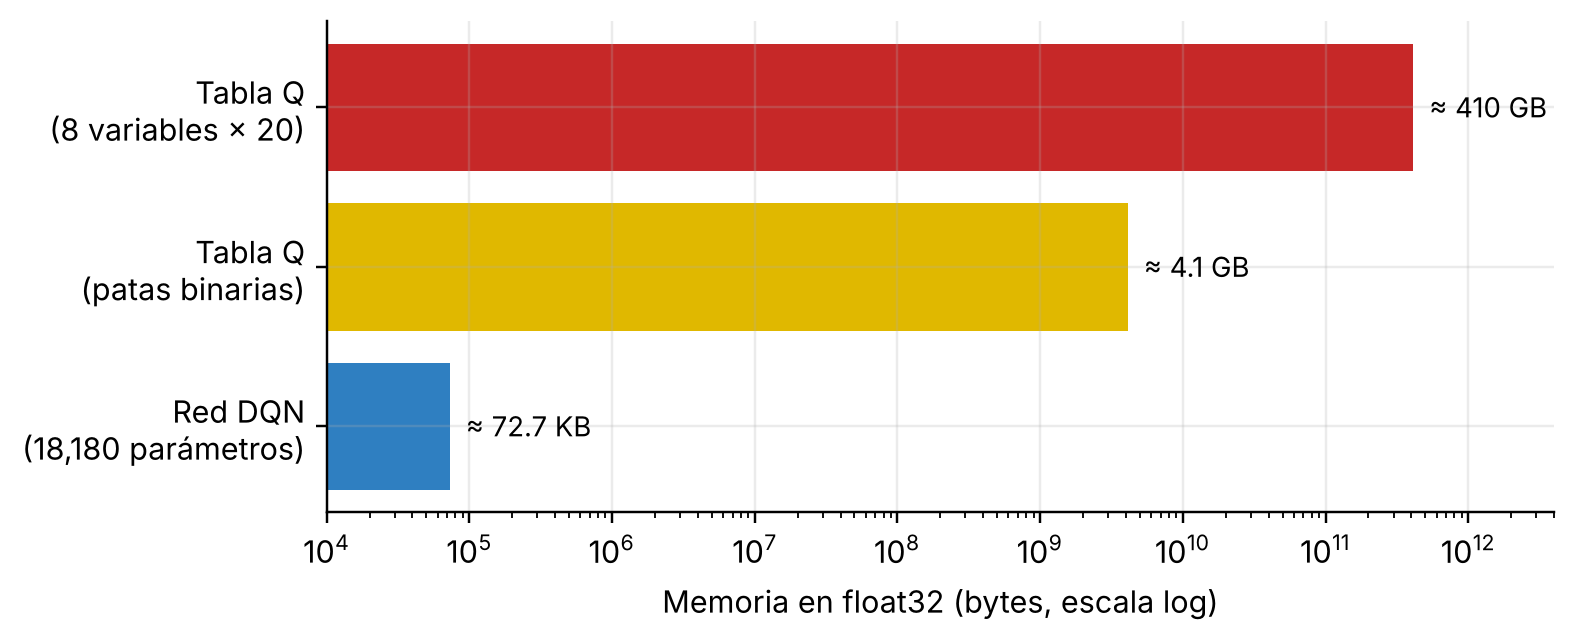
\includegraphics[width=0.78\textwidth]{images/escalabilidad.png}
\caption{Comparación de memoria en escala logarítmica.}
\label{fig:escalabilidad}
\end{figure}

La memoria es solo la mitad del problema. Una tabla necesita \emph{visitar} cada
celda muchas veces para estimarla, y con $10^8$ a $10^{10}$ estados casi todas
quedarían sin datos; además, con 20 segmentos la física se vuelve ``pixelada''
(el ángulo cambiaría en saltos de $\sim 18^\circ$). La red \textbf{generaliza}:
estados cercanos comparten pesos, así que lo aprendido en uno se transfiere a sus
vecinos. Por eso bastaron unos $500$ episodios en lugar de miles de millones de
visitas, lo que justifica el aproximador neuronal.

\subsection{Validación del port de LunarLander}

Para que el juego del sitio sea fiel al experimento, se comparó el port en
\texttt{planck.js} contra Gymnasium con $100$ episodios por lado. Como los
generadores aleatorios son distintos, los terrenos no coinciden y se comparan
distribuciones.

\begin{table}[H]
\centering
\renewcommand{\arraystretch}{1.2}
\begin{tabular}{|l|c|c|}
\hline
\rowcolor{iberoblue}
\textcolor{white}{Controlador} & \textcolor{white}{Gymnasium (Python, Box2D)} &
\textcolor{white}{Navegador (planck.js)} \\ \hline
Heurística de Gymnasium   & $252.8 \pm 73.1$, $95\%$ aterrizajes & $255.3 \pm 67.8$, $97\%$ aterrizajes \\ \hline
DQN (red principal)       & $193.3 \pm 59.5$, $77\%$ aterrizajes & $196.4 \pm 63.6$, $76\%$ aterrizajes \\ \hline
DQN sin costo$^{*}$       & $229.8 \pm 80.5$, $70\%$ aterrizajes & $219.0 \pm 83.3$, $62\%$ aterrizajes \\ \hline
\end{tabular}
\caption{Validación estadística del port. $^{*}$Evaluada con la recompensa sin
costo de combustible con la que se entrenó.}
\label{tbl:validacion}
\end{table}

Las diferencias están dentro del ruido de 100 episodios, lo que confirma que la
red entrenada en Python se comporta igual en el navegador.

\section{Discusión}

\begin{itemize}
    \item \textbf{On-policy frente a off-policy es una actitud ante el riesgo.}
    Con el mismo mapa, los mismos hiperparámetros y las mismas semillas, la
    única diferencia en el código es una línea (el blanco TD), y basta para que
    los agentes elijan rutas opuestas. Q-learning aprende lo que es óptimo
    \emph{si no hubiera errores}; SARSA, lo que es óptimo \emph{dado que sí los
    habrá}.

    \item \textbf{El ruido es lo que separa a los algoritmos.} Sin resbalón ni
    exploración, ambos convergerían a la ruta corta. El resbalón afecta a los dos
    por igual, porque es parte del entorno; la exploración solo la ``ve'' SARSA.
    Por eso el mapa de calor se midió con $\varepsilon = 0.1$: con la política
    greedy pura la diferencia de riesgo casi desaparece.

    \item \textbf{El diseño del mapa importa.} Las primeras versiones del mapa,
    con una brecha de tres celdas en diagonal, eran tan difíciles de descubrir
    con $\varepsilon$ constante que Q-learning nunca encontraba el atajo. Se usó
    programación dinámica para elegir una geometría donde la política óptima
    greedy cruza la brecha y la $\varepsilon$-suave la rodea, y después se
    comprobó con entrenamiento real en las 5 semillas. Aun así, una semilla de
    Q-learning nunca encontró la brecha, lo que muestra la limitación de una
    exploración $\varepsilon$-greedy sin decaimiento.

    \item \textbf{El criterio de paro de DQN es engañoso.} Detener el
    entrenamiento justo al cruzar la media móvil de 200 deja una política greedy
    que todavía conserva el hábito de flotar. La media de entrenamiento incluye
    el efecto de $\varepsilon$, que saca al módulo del \emph{hover}. Una
    evaluación greedy con más episodios, o seguir entrenando con $\varepsilon$
    mínimo, da una imagen más fiel.

    \item \textbf{La recompensa moldea el comportamiento.} Quitar el costo de
    combustible no cambia el objetivo de aterrizar, pero duplica el uso del motor
    principal. El agente optimiza exactamente lo que se le pide, no lo que el
    diseñador ``quiso decir''.
\end{itemize}

\section{Conclusiones}

\begin{enumerate}
    \item Se modeló la navegación del robot como un MDP de $400$ estados y $8$
    acciones con resbalamiento, y se diseñó el mapa \emph{El Paso del
    Contrabandista}, con una brecha diagonal de una celda y un rodeo seguro.
    \item Durante el entrenamiento, SARSA converge a una recompensa más alta
    ($72.7 \pm 3.3$ contra $62.3 \pm 8.5$) porque considera la exploración en su
    blanco TD. Q-learning aprende el camino óptimo pero cae más con
    $\varepsilon$: $10.2\%$ de choques contra $1.1\%$.
    \item Se verificó la hipótesis de los mapas de calor: Q-learning corta por la
    brecha en el $74\%$ de los episodios, mientras que SARSA la rodea con un
    colchón de seguridad.
    \item Para un robot costoso entre personas se recomienda SARSA por su
    aversión al riesgo: sacrifica algo de recompensa esperada a cambio de reducir
    mucho la probabilidad de un fallo catastrófico.
    \item El agente DQN superó la media móvil de $+200$ en el episodio $526$ en
    unos dos minutos de CPU, pasando por cuatro fases identificables. La
    evaluación greedy dio $160.9 \pm 79.6$ en 20 episodios y $193.3 \pm 59.5$ en
    100; con cuatro semillas, el promedio fue $193.2$.
    \item La penalización por combustible induce una política eficiente; sin
    ella, el agente duplica el uso del motor principal y su puntaje real cae de
    $160.9$ a $128.1$.
    \item Una tabla Q discretizada requeriría entre $4.1$~GB y $410$~GB, de
    $5.6 \times 10^4$ a $5.6 \times 10^6$ veces más que los $18{,}180$ parámetros
    de la red. Esto, junto con la necesidad de visitar cada celda, justifica el
    aproximador neuronal.
    \item Se desarrolló un sitio interactivo con despliegue automático y dos
    juegos 3D que usan los resultados reales. En particular, la red DQN pilota en
    el navegador sobre un port de la física validado contra Gymnasium.
\end{enumerate}

\section*{Declaración sobre el uso de inteligencia artificial}

Durante el desarrollo de esta práctica se utilizó Claude (Anthropic, 2026) como
herramienta de apoyo en la programación de los agentes, del sitio web y de los
juegos 3D, en el port de la física de LunarLander, en la configuración del
despliegue en GitHub Pages, en la generación de las figuras y en la redacción y
estructuración de este documento. La formulación del problema, la verificación
de los resultados y la revisión del contenido fueron realizadas y validadas por
los autores.

\section{Referencias}

\begin{itemize}
    \item Sutton, R. S., \& Barto, A. G. (2018). \emph{Reinforcement Learning: An
    Introduction} (2a~ed.). MIT Press. Capítulo 6; ejemplo 6.6, \emph{Cliff
    Walking}.
    \item Watkins, C. J. C. H., \& Dayan, P. (1992). Q-learning. \emph{Machine
    Learning}, 8(3--4), 279--292.
    \item Rummery, G. A., \& Niranjan, M. (1994). \emph{On-line Q-learning using
    connectionist systems} (Reporte técnico CUED/F-INFENG/TR 166). Universidad de
    Cambridge.
    \item Lin, L.-J. (1992). Self-improving reactive agents based on reinforcement
    learning, planning and teaching. \emph{Machine Learning}, 8(3--4), 293--321.
    \item Mnih, V., Kavukcuoglu, K., Silver, D., et al. (2015). Human-level control
    through deep reinforcement learning. \emph{Nature}, 518(7540), 529--533.
    \item Towers, M., et al. (2024). \emph{Gymnasium: A Standard Interface for
    Reinforcement Learning Environments}. arXiv:2407.17032.
    \url{https://gymnasium.farama.org}
    \item Paszke, A., et al. (2019). PyTorch: An imperative style,
    high-performance deep learning library. \emph{Advances in Neural Information
    Processing Systems}, 32.
    \item López González, A., \& Caballero Mora, J. (2026). \emph{Práctica Sarsa,
    Q-learning y Deep Q-learning} [Material del curso]. Universidad
    Iberoamericana.
    \item Anthropic. (2026). \emph{Claude} (Opus 5) [Modelo de lenguaje de gran
    escala]. \url{https://claude.ai}
\end{itemize}

\end{document}
